\documentclass[12pt, a4paper]{article}

% ── Packages ──────────────────────────────────────────────
\usepackage[utf8]{inputenc}
\usepackage[T1]{fontenc}
\usepackage{amsmath, amssymb, amsthm}
\usepackage{graphicx}
\usepackage{hyperref}
\usepackage{booktabs}
\usepackage{geometry}
\usepackage{caption}
\usepackage{subcaption}
\usepackage{xcolor}
\usepackage{listings}
\usepackage{float}

\geometry{margin=1in}
\hypersetup{
    colorlinks=true,
    linkcolor=blue!70!black,
    citecolor=green!50!black,
    urlcolor=blue!60!black
}

% ── Listing style for Python ─────────────────────────────
\lstset{
    language=Python,
    basicstyle=\ttfamily\small,
    keywordstyle=\color{blue}\bfseries,
    commentstyle=\color{green!50!black}\itshape,
    stringstyle=\color{red!60!black},
    numbers=left,
    numberstyle=\tiny\color{gray},
    frame=single,
    breaklines=true,
    captionpos=b
}

% ── Title ─────────────────────────────────────────────────
\title{%
    \textbf{Validate Sampling via Monte Carlo Simulation}\\[6pt]
    \large Demonstrating the Law of Large Numbers
}
\author{Monte Carlo Simulation Notebook}
\date{February 2026}

\begin{document}
\maketitle

% ══════════════════════════════════════════════════════════
\begin{abstract}
This document accompanies the Jupyter notebook
\texttt{MonteCarloSimulation.ipynb}.  We sample from several
probability distributions, compute the running sample average of a
target function~$f$, and show empirically that the sample average
converges to the true expectation as the number of samples grows---a
direct illustration of the \emph{Law of Large Numbers}.
\end{abstract}

\tableofcontents
\newpage

% ══════════════════════════════════════════════════════════
\section{Introduction}
\label{sec:intro}

Given a random variable $X$ distributed according to a probability
density (or mass) function $p(x)$ and a measurable function $f$, the
\emph{expectation} of $f(X)$ is

\begin{equation}
    E[f(X)] \;=\; \int_{-\infty}^{\infty} f(x)\, p(x)\, dx
    \label{eq:expectation}
\end{equation}

\noindent for continuous distributions, or the analogous sum for
discrete distributions.

\subsection{Monte Carlo Estimator}

The Monte Carlo estimate draws $N$ i.i.d.\ samples
$x_1, x_2, \ldots, x_N \sim p(x)$ and computes

\begin{equation}
    \hat{\mu}_N \;=\; \frac{1}{N} \sum_{i=1}^{N} f(x_i)
    \label{eq:mc_estimator}
\end{equation}

By the \textbf{Strong Law of Large Numbers},

\begin{equation}
    \hat{\mu}_N \;\xrightarrow{\text{a.s.}}\; E[f(X)]
    \quad\text{as } N \to \infty
    \label{eq:lln}
\end{equation}

Moreover, by the \textbf{Central Limit Theorem}, the estimation error
is normally distributed for large $N$:

\begin{equation}
    \hat{\mu}_N - E[f(X)] \;\approx\;
    \mathcal{N}\!\left(0,\;\frac{\sigma_f^2}{N}\right),
    \qquad
    \sigma_f^2 = \mathrm{Var}[f(X)]
    \label{eq:clt}
\end{equation}

This means the standard error shrinks as $O(1/\sqrt{N})$.

% ══════════════════════════════════════════════════════════
\section{Example 1: Normal Distribution --- Estimate \texorpdfstring{$E[X^2]$}{E[X²]}}
\label{sec:ex1}

\subsection{Setup}

Let $X \sim \mathcal{N}(\mu, \sigma^2)$ with $\mu = 2$ and
$\sigma = 3$.  We choose $f(x) = x^2$ and estimate $E[X^2]$.

\subsection{Analytical Solution}

\begin{equation}
    E[X^2] = \mu^2 + \sigma^2 = 4 + 9 = 13
\end{equation}

\subsection{Experiment}

We draw $N = 10{,}000$ samples from $\mathcal{N}(2, 9)$, apply
$f(x) = x^2$, and plot the running average $\hat{\mu}_N$ against the
true value.

\begin{figure}[H]
    \centering
    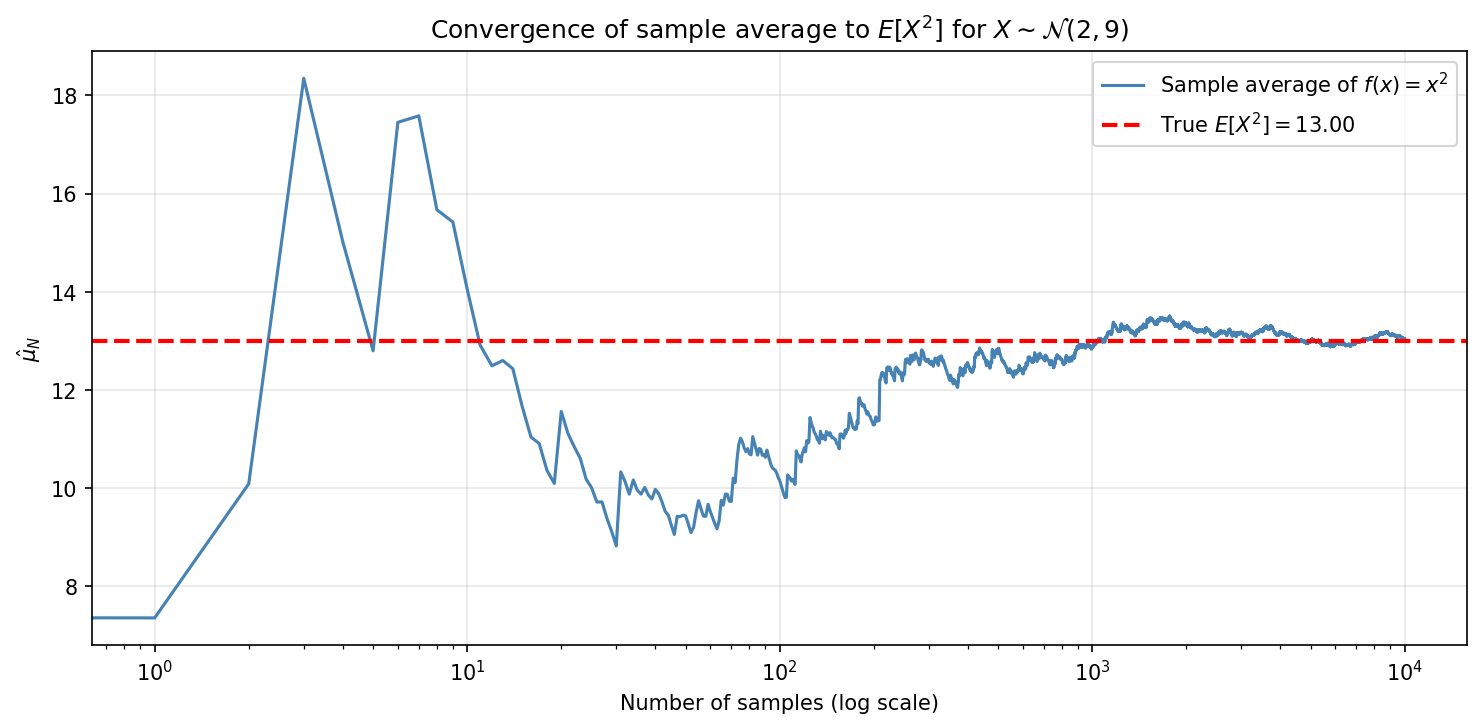
\includegraphics[width=0.92\textwidth]{images/ex1_normal_convergence.png}
    \caption{Convergence of the sample average of $f(x)=x^2$ to
             $E[X^2]=13$ for $X \sim \mathcal{N}(2,9)$.
             The red dashed line marks the true expectation.}
    \label{fig:ex1}
\end{figure}

\subsection{Results}

\begin{table}[H]
    \centering
    \begin{tabular}{lr}
        \toprule
        \textbf{Quantity} & \textbf{Value} \\
        \midrule
        True $E[X^2]$                & 13.0000 \\
        Estimate ($N=10{,}000$)      & 13.0359 \\
        Absolute error               &  0.0359 \\
        \bottomrule
    \end{tabular}
    \caption{Numerical results for Example~1.}
    \label{tab:ex1}
\end{table}

% ══════════════════════════════════════════════════════════
\section{Example 2: Exponential Distribution --- Estimate \texorpdfstring{$E[\sin(X)]$}{E[sin(X)]}}
\label{sec:ex2}

\subsection{Setup}

Let $X \sim \mathrm{Exp}(\lambda)$ with rate $\lambda = 1.5$, so that
$p(x) = \lambda e^{-\lambda x}$ for $x \ge 0$.  We estimate
$E[\sin(X)]$.

\subsection{Analytical Solution}

Using the Laplace transform of $\sin$:

\begin{equation}
    E[\sin(X)] = \int_0^{\infty} \sin(x)\,\lambda e^{-\lambda x}\,dx
               = \frac{\lambda}{\lambda^2 + 1}
               = \frac{1.5}{1.5^2 + 1}
               = \frac{1.5}{3.25}
               \approx 0.4615
\end{equation}

\subsection{Experiment}

\begin{figure}[H]
    \centering
    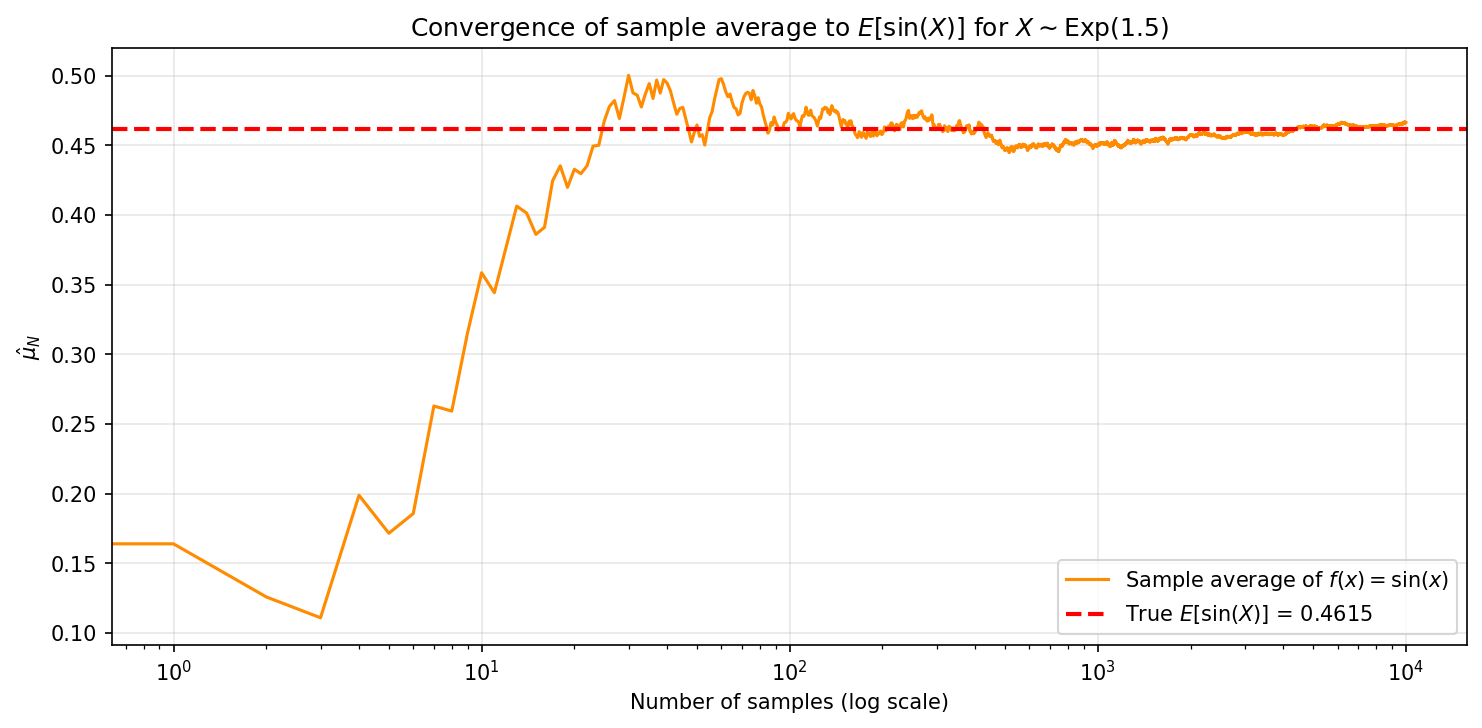
\includegraphics[width=0.92\textwidth]{images/ex2_exponential_convergence.png}
    \caption{Convergence of the sample average of $f(x)=\sin(x)$ to
             $E[\sin(X)] \approx 0.4615$ for $X \sim \mathrm{Exp}(1.5)$.}
    \label{fig:ex2}
\end{figure}

\subsection{Results}

\begin{table}[H]
    \centering
    \begin{tabular}{lr}
        \toprule
        \textbf{Quantity} & \textbf{Value} \\
        \midrule
        True $E[\sin(X)]$           & 0.4615 \\
        Estimate ($N=10{,}000$)     & 0.4663 \\
        Absolute error              & 0.0047 \\
        \bottomrule
    \end{tabular}
    \caption{Numerical results for Example~2.}
    \label{tab:ex2}
\end{table}

% ══════════════════════════════════════════════════════════
\section{Example 3: Multiple Trials --- Confidence Envelope}
\label{sec:ex3}

\subsection{Motivation}

A single trajectory only shows \emph{one} realization of the
convergence.  By running 50 independent trials we can visualize the
\emph{spread} of the estimator and compare it with the theoretical
standard error.

\subsection{Theoretical Standard Error}

For $f(x) = x^2$ and $X \sim \mathcal{N}(\mu, \sigma^2)$:

\begin{align}
    E[X^4] &= \mu^4 + 6\mu^2\sigma^2 + 3\sigma^4 \\
    \mathrm{Var}[f(X)] &= E[X^4] - (E[X^2])^2 \\
    \mathrm{SE}(\hat{\mu}_N) &= \sqrt{\frac{\mathrm{Var}[f(X)]}{N}}
\end{align}

\subsection{Experiment}

\begin{figure}[H]
    \centering
    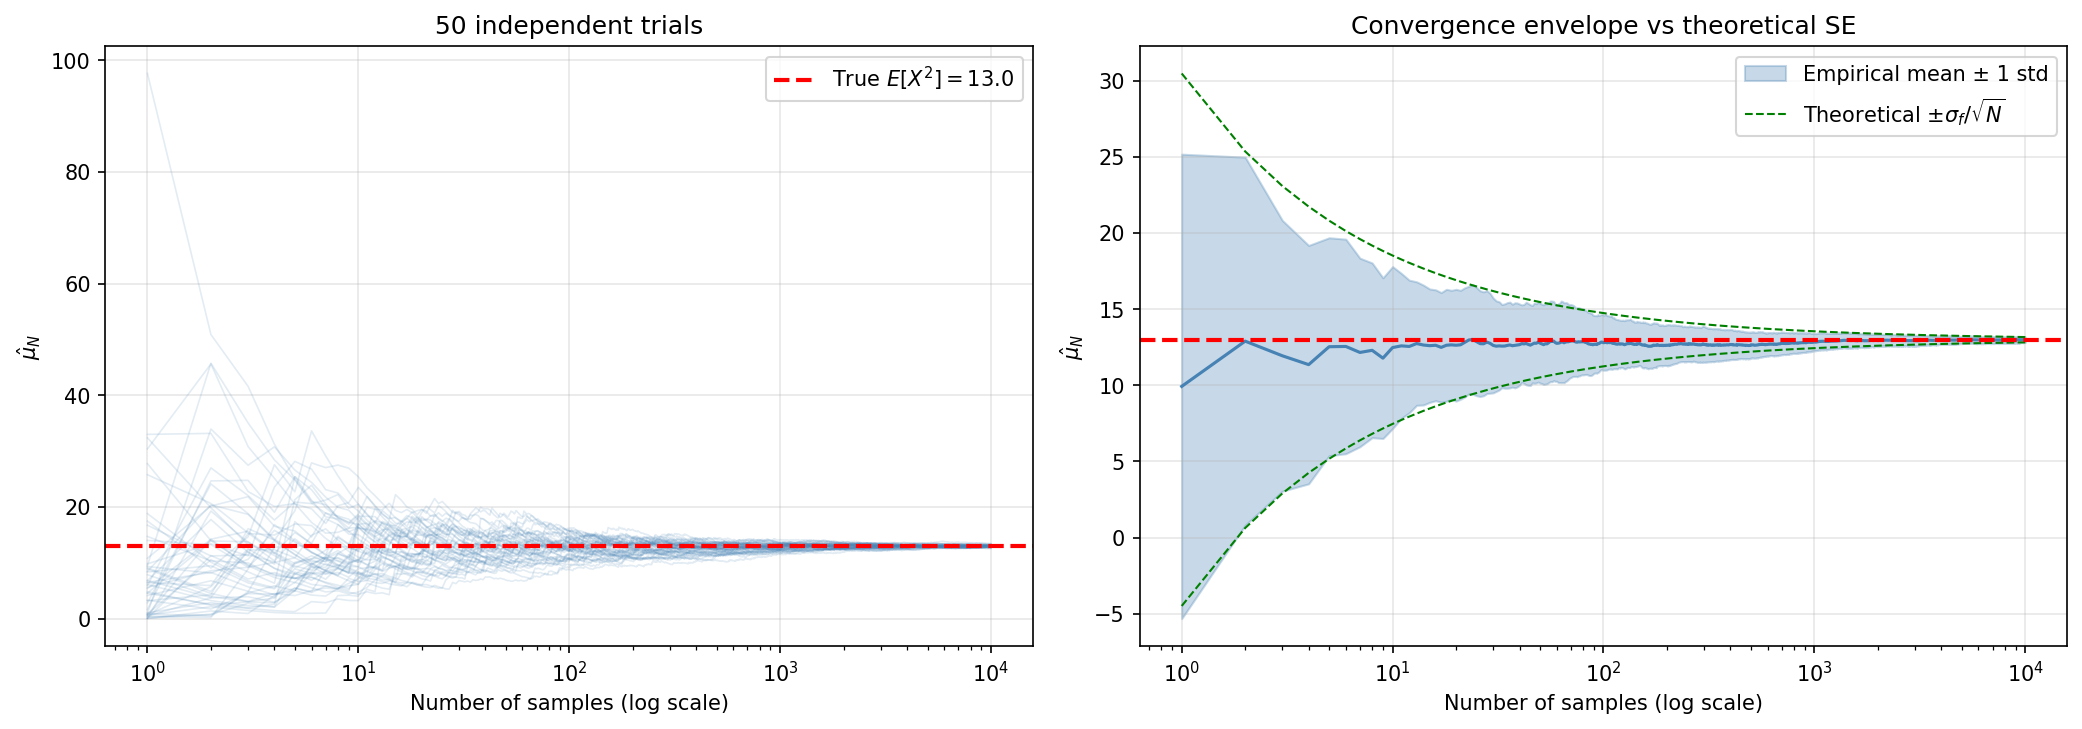
\includegraphics[width=\textwidth]{images/ex3_confidence_envelope.png}
    \caption{\textbf{Left:} 50 independent trial trajectories converging
             to $E[X^2]=13$.
             \textbf{Right:} Empirical mean $\pm$ 1 standard deviation
             (blue band) overlaid with the theoretical standard error
             envelope (green dashed).}
    \label{fig:ex3}
\end{figure}

The green dashed theoretical envelope closely matches the empirical
spread, confirming the $O(1/\sqrt{N})$ convergence rate predicted by
the Central Limit Theorem.

% ══════════════════════════════════════════════════════════
\section{Example 4: Discrete Distribution --- Custom PMF}
\label{sec:ex4}

\subsection{Setup}

Define a discrete random variable $X$ taking values in
$\{1, 2, 3, 4, 5\}$ with probability mass function:

\begin{table}[H]
    \centering
    \begin{tabular}{cccccc}
        \toprule
        $x$    & 1    & 2    & 3    & 4    & 5    \\
        $p(x)$ & 0.10 & 0.20 & 0.30 & 0.25 & 0.15 \\
        \bottomrule
    \end{tabular}
    \caption{Probability mass function for the discrete example.}
    \label{tab:pmf}
\end{table}

We estimate $E[X^2]$ using $f(x) = x^2$.

\subsection{Analytical Solution}

\begin{equation}
    E[X^2] = \sum_{x=1}^{5} x^2 \, p(x)
           = 1(0.10) + 4(0.20) + 9(0.30) + 16(0.25) + 25(0.15)
           = 11.35
\end{equation}

\subsection{Experiment}

\begin{figure}[H]
    \centering
    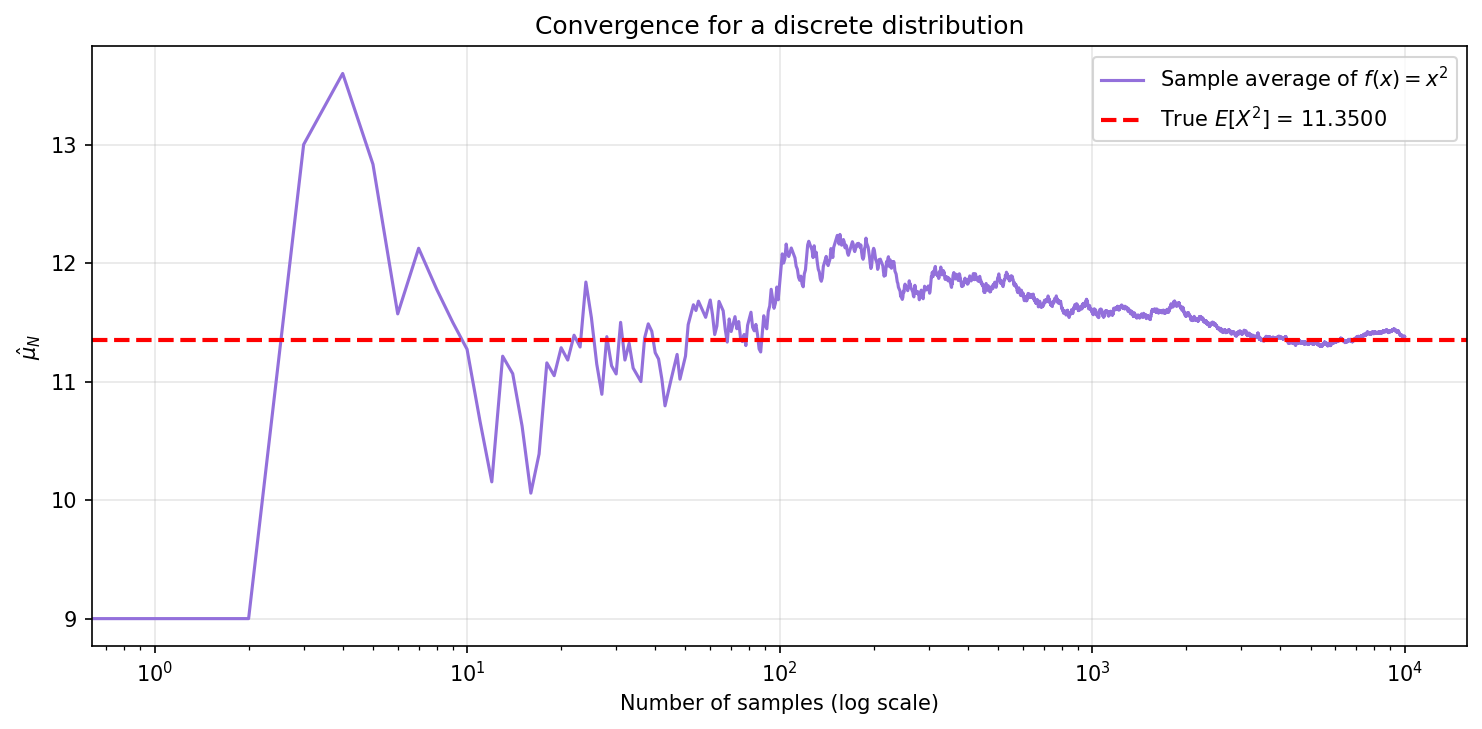
\includegraphics[width=0.92\textwidth]{images/ex4_discrete_convergence.png}
    \caption{Convergence of the sample average to $E[X^2]=11.35$ for the
             discrete distribution.}
    \label{fig:ex4}
\end{figure}

\subsection{Results}

\begin{table}[H]
    \centering
    \begin{tabular}{lr}
        \toprule
        \textbf{Quantity} & \textbf{Value} \\
        \midrule
        True $E[X^2]$               & 11.3500 \\
        Estimate ($N=10{,}000$)     & 11.3819 \\
        Absolute error              &  0.0319 \\
        \bottomrule
    \end{tabular}
    \caption{Numerical results for Example~4.}
    \label{tab:ex4}
\end{table}

% ══════════════════════════════════════════════════════════
\section{Sampling from a Distribution}
\label{sec:sampling}

The Monte Carlo examples above assume we can draw samples directly from
the target distribution~$p(x)$.  In practice the target may be known
only up to a normalizing constant, or sampling from it directly may be
infeasible.  \emph{Sampling methods} bridge this gap by transforming
easy-to-obtain random variates into draws that follow the desired
distribution.

Several widely used families are:
\begin{itemize}
    \item \textbf{Rejection sampling} — accept/reject proposals from a
          simpler distribution.
    \item \textbf{Importance sampling} — re-weight samples from a
          proposal to estimate expectations under the target.
    \item \textbf{Markov-chain Monte Carlo (MCMC)} — construct a Markov
          chain whose stationary distribution is the target.
\end{itemize}

% ──────────────────────────────────────────────────────────
\subsection{Rejection Sampling}
\label{sec:rejection}

\subsubsection{Algorithm}

Suppose we wish to sample from an unnormalized target density
$\tilde{p}(z)$ (i.e.\ $p(z) = \tilde{p}(z)/Z_p$ where the
normalizing constant $Z_p$ may be unknown).

\begin{enumerate}
    \item Choose a \textbf{proposal distribution}~$q(z)$ that is easy
          to sample from and whose support covers that of
          $\tilde{p}(z)$.
    \item Find a constant $k$ such that
          \begin{equation}
              k\,q(z) \;\geq\; \tilde{p}(z) \qquad \forall\, z.
              \label{eq:envelope}
          \end{equation}
    \item Repeat:
          \begin{enumerate}
              \item Draw $z_0 \sim q(z)$.
              \item Draw $u_0 \sim \mathrm{Uniform}(0,\; k\,q(z_0))$.
              \item \textbf{Accept} $z_0$ if $u_0 \leq \tilde{p}(z_0)$;
                    otherwise \textbf{reject} and return to step~(a).
          \end{enumerate}
\end{enumerate}

The accepted samples are distributed according to the normalized
target~$p(z)$.  The \textbf{acceptance rate} equals
$Z_p / k$, so a tight envelope (small~$k$) is essential for
efficiency.

\subsubsection{Experimental Setup}

We define a multimodal unnormalized target:
\begin{equation}
    \tilde{p}(z) \;=\;
        \exp\!\Bigl(-\tfrac{1}{2}(z-2)^2\Bigr)
        \;+\;
        0.5\,\exp\!\bigl(-0.2\,(z+3)^2\bigr)\,\sin^2(3z)
    \label{eq:target}
\end{equation}

\begin{itemize}
    \item The first component is a Gaussian bump centred at $z=2$.
    \item The second component is an oscillatory, Gaussian-modulated
          bump near $z=-3$.
\end{itemize}

The proposal is a wide Gaussian $q(z) = \mathcal{N}(z \mid 0,\, 16)$
($\sigma = 4$).  The bounding constant is set to
$k = 1.1 \times \max_z \bigl[\tilde{p}(z)/q(z)\bigr]$, computed over
a dense grid with a 10\% safety margin, yielding $k \approx 12.60$.

\begin{lstlisting}[caption={Python implementation of rejection sampling.},
                   label=lst:rejection]
import numpy as np
from scipy.stats import norm

def p_tilde(z):
    return (
        np.exp(-0.5*(z - 2)**2)
        + 0.5*np.exp(-0.2*(z + 3)**2)*np.sin(3*z)**2
    )

def q(z):
    return norm.pdf(z, loc=0, scale=4)

def sample_q():
    return np.random.normal(0, 4)

# Compute bounding constant k
z_grid = np.linspace(-15, 15, 100000)
k = np.max(p_tilde(z_grid) / q(z_grid))
k *= 1.1  # 10% safety margin

def rejection_sampling(N):
    samples = []
    attempts = 0
    while len(samples) < N:
        z0 = sample_q()
        u0 = np.random.uniform(0, k * q(z0))
        attempts += 1
        if u0 <= p_tilde(z0):
            samples.append(z0)
    return np.array(samples), attempts

samples, attempts = rejection_sampling(10000)
print(f"Acceptance rate: {len(samples)/attempts:.3f}")
\end{lstlisting}

\subsubsection{Target vs.\ Proposal Envelope}

Figure~\ref{fig:rs_envelope} shows the unnormalized target alongside
the scaled proposal $k\,q(z)$.  The shaded region represents the
``rejection zone''---proposals falling there are discarded.

\begin{figure}[H]
    \centering
    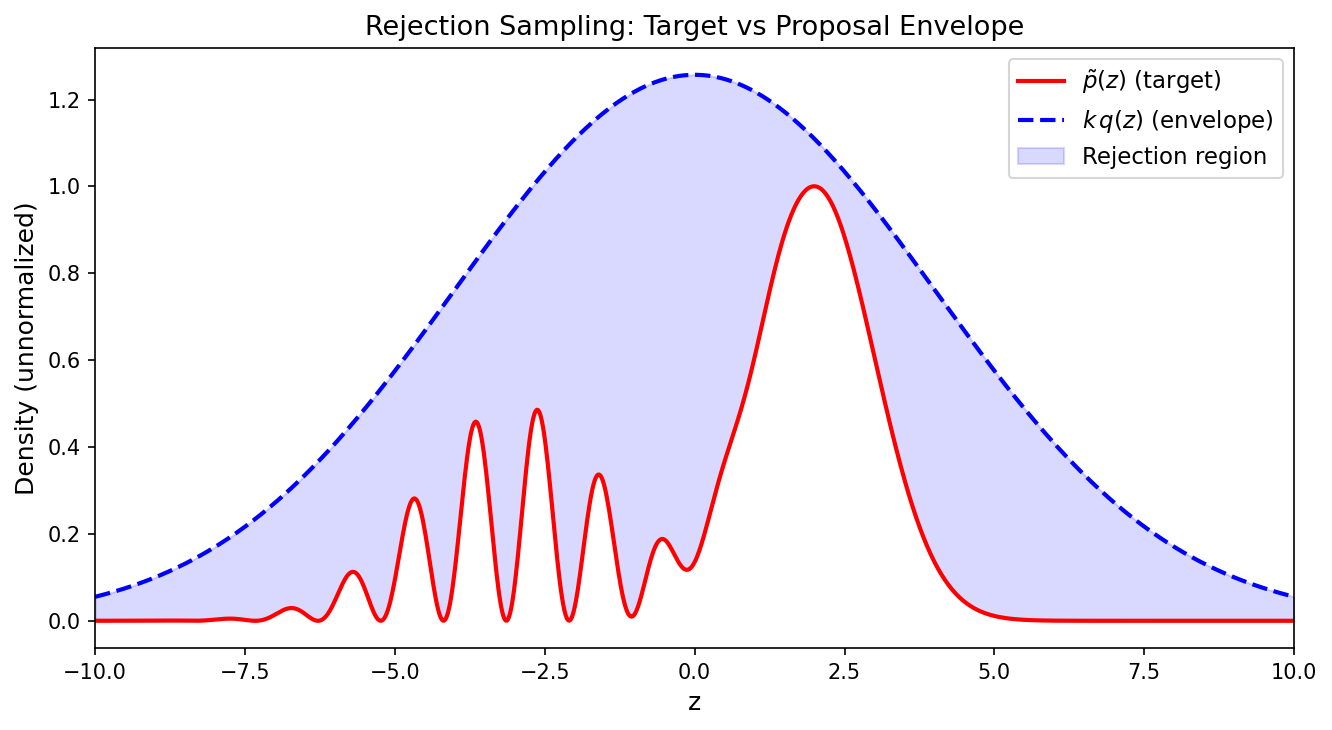
\includegraphics[width=0.92\textwidth]{images/rejection_sampling_envelope.png}
    \caption{Unnormalized target $\tilde{p}(z)$ (red) versus the
             proposal envelope $k\,q(z)$ (blue dashed).  The blue
             shaded area is the rejection region.}
    \label{fig:rs_envelope}
\end{figure}

\subsubsection{Results}

We generate $N = 10{,}000$ accepted samples via rejection sampling.

\begin{table}[H]
    \centering
    \begin{tabular}{lr}
        \toprule
        \textbf{Quantity} & \textbf{Value} \\
        \midrule
        Accepted samples             & 10{,}000 \\
        Total proposals              & $\approx$\,36{,}000 \\
        Acceptance rate              & $\approx 27.7\%$ \\
        Bounding constant $k$        & 12.60 \\
        \bottomrule
    \end{tabular}
    \caption{Rejection sampling statistics.}
    \label{tab:rs}
\end{table}

Figure~\ref{fig:rs_result} overlays the histogram of accepted samples
with the true (numerically normalized) target density.  The close match
confirms that rejection sampling correctly reproduces the target.

\begin{figure}[H]
    \centering
    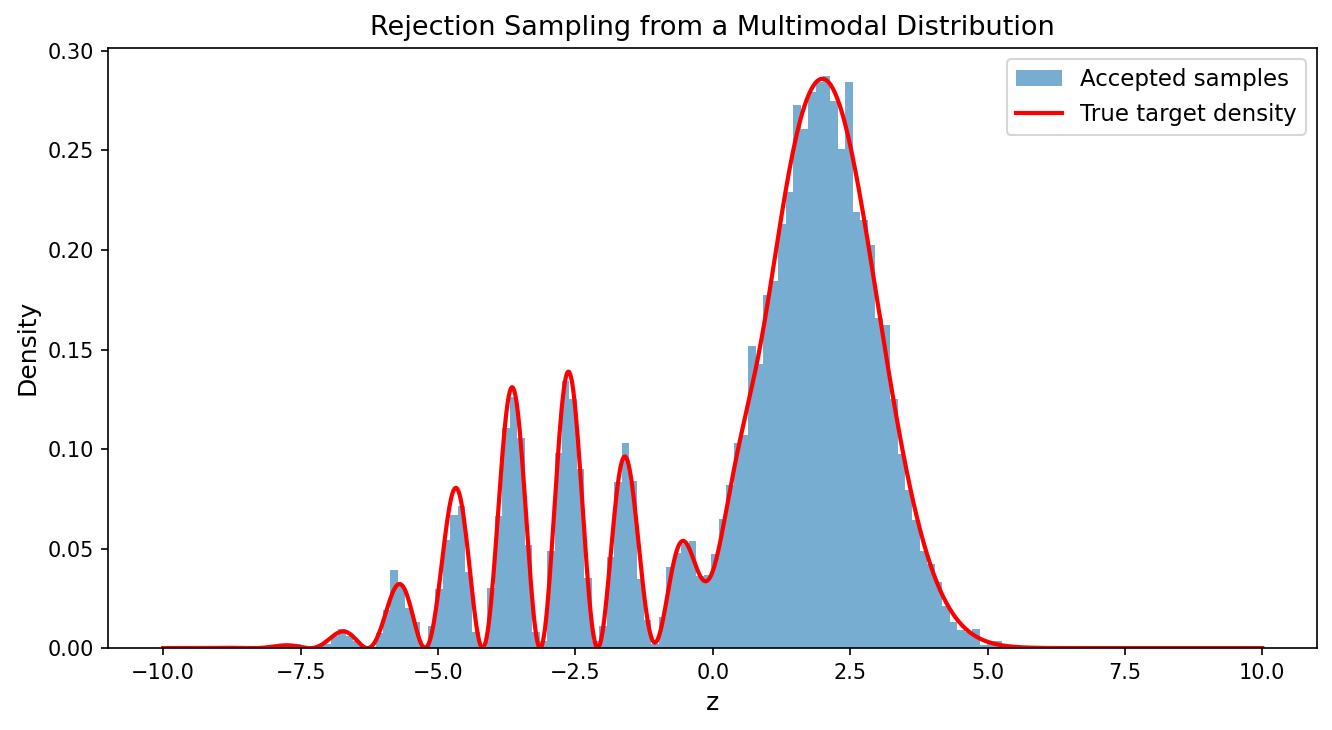
\includegraphics[width=0.92\textwidth]{images/rejection_sampling_result.png}
    \caption{Histogram of $10{,}000$ accepted samples versus the
             normalized target density $p(z)$.  The agreement validates
             the rejection sampler.}
    \label{fig:rs_result}
\end{figure}

\subsubsection{Discussion}

\begin{itemize}
    \item The acceptance rate of $\approx 27.7\%$ is reasonable for a
          one-dimensional problem but would degrade exponentially in
          higher dimensions.
    \item The grid-based computation of $k$ is practical here; for
          sharply peaked targets a coarse grid could underestimate $k$
          and bias the results.
    \item For high-dimensional or strongly peaked targets, methods such
          as \emph{Importance Sampling} or \emph{MCMC} (e.g.\
          Metropolis--Hastings, Hamiltonian Monte Carlo) are preferred.
\end{itemize}

% ──────────────────────────────────────────────────────────
\subsection{Importance Sampling}
\label{sec:importance}

While rejection sampling discards proposals that fall outside the
target envelope, \textbf{importance sampling} keeps \emph{every}
proposal and instead assigns each sample a \emph{weight} that
corrects for the mismatch between the proposal and the target.
This makes it especially useful when samples are expensive to
generate.

\subsubsection{Algorithm}

Given an unnormalized target $\tilde{p}(z)$ and a proposal
distribution $q(z)$ from which we can sample:

\begin{enumerate}
    \item Draw $L$ samples
          $z^{(1)}, z^{(2)}, \ldots, z^{(L)} \sim q(z)$.
    \item Compute \textbf{unnormalized importance weights}:
          \begin{equation}
              \tilde{r}^{(\ell)} \;=\;
              \frac{\tilde{p}\bigl(z^{(\ell)}\bigr)}
                   {q\bigl(z^{(\ell)}\bigr)}
              \label{eq:is_unnorm}
          \end{equation}
    \item \textbf{Normalize} the weights (self-normalized variant):
          \begin{equation}
              w^{(\ell)} \;=\;
              \frac{\tilde{r}^{(\ell)}}
                   {\sum_{j=1}^{L} \tilde{r}^{(j)}}
              \label{eq:is_norm}
          \end{equation}
    \item Estimate the expectation:
          \begin{equation}
              \hat{E}_p[f(z)] \;=\;
              \sum_{\ell=1}^{L} w^{(\ell)}\, f\bigl(z^{(\ell)}\bigr)
              \label{eq:is_estimate}
          \end{equation}
\end{enumerate}

\paragraph{Why it works.}
The key identity is
\begin{equation}
    E_p[f(z)]
    = \int f(z)\,p(z)\,dz
    = \int f(z)\,\frac{p(z)}{q(z)}\,q(z)\,dz
    = E_q\!\left[f(z)\,\frac{p(z)}{q(z)}\right]
    \label{eq:is_identity}
\end{equation}
When $p$ is known only up to a constant
($p(z) = \tilde{p}(z)/Z_p$), the self-normalized estimator
(Equations~\ref{eq:is_norm}--\ref{eq:is_estimate}) avoids
needing~$Z_p$.

\paragraph{Effective Sample Size.}
A useful diagnostic for weight quality is the \textbf{effective
sample size} (ESS):
\begin{equation}
    \mathrm{ESS} \;=\;
    \frac{1}{\sum_{\ell=1}^{L}\bigl(w^{(\ell)}\bigr)^2}
    \label{eq:ess}
\end{equation}
An ESS close to $L$ indicates nearly uniform weights (good);
an ESS close to 1 means a single sample dominates (bad).

\subsubsection{Experiment~1: Single Gaussian Proposal}

\paragraph{Setup.}
\begin{table}[H]
    \centering
    \begin{tabular}{ll}
        \toprule
        \textbf{Component} & \textbf{Definition} \\
        \midrule
        Unnormalized target
            & $\tilde{p}(z) = \exp(-z^4 + 2z^2)$
              — bimodal, peaks near $z = \pm 1$ \\
        Proposal
            & $q(z) = \mathcal{N}(0,\, 4)$
              — single wide Gaussian ($\sigma = 2$) \\
        Function of interest
            & $f(z) = z^2$ \\
        Number of samples
            & $L = 100{,}000$ \\
        \bottomrule
    \end{tabular}
    \caption{Importance sampling setup --- single Gaussian proposal.}
    \label{tab:is1_setup}
\end{table}

A single Gaussian centred at $z = 0$ covers both modes of the target
but wastes probability mass in the valley between them.  This leads
to a broader spread of importance weights and a lower ESS.

\begin{lstlisting}[caption={Importance sampling with a single Gaussian proposal.},
                   label=lst:is_single]
import numpy as np

def p_tilde(z):
    return np.exp(-z**4 + 2*z**2)

sigma = 2.0

def q_tilde(z):
    return np.exp(-0.5 * (z / sigma)**2)

def f(z):
    return z**2

np.random.seed(0)
L = 100_000

# Step 1: sample from q(z)
z_samples = np.random.normal(0, sigma, size=L)

# Step 2: unnormalized importance weights
r_tilde = p_tilde(z_samples) / q_tilde(z_samples)

# Step 3: normalize weights
weights = r_tilde / np.sum(r_tilde)

# Step 4: estimate expectation
E_f = np.sum(weights * f(z_samples))
print("Estimated E_p[z^2] =", E_f)
\end{lstlisting}

\begin{figure}[H]
    \centering
    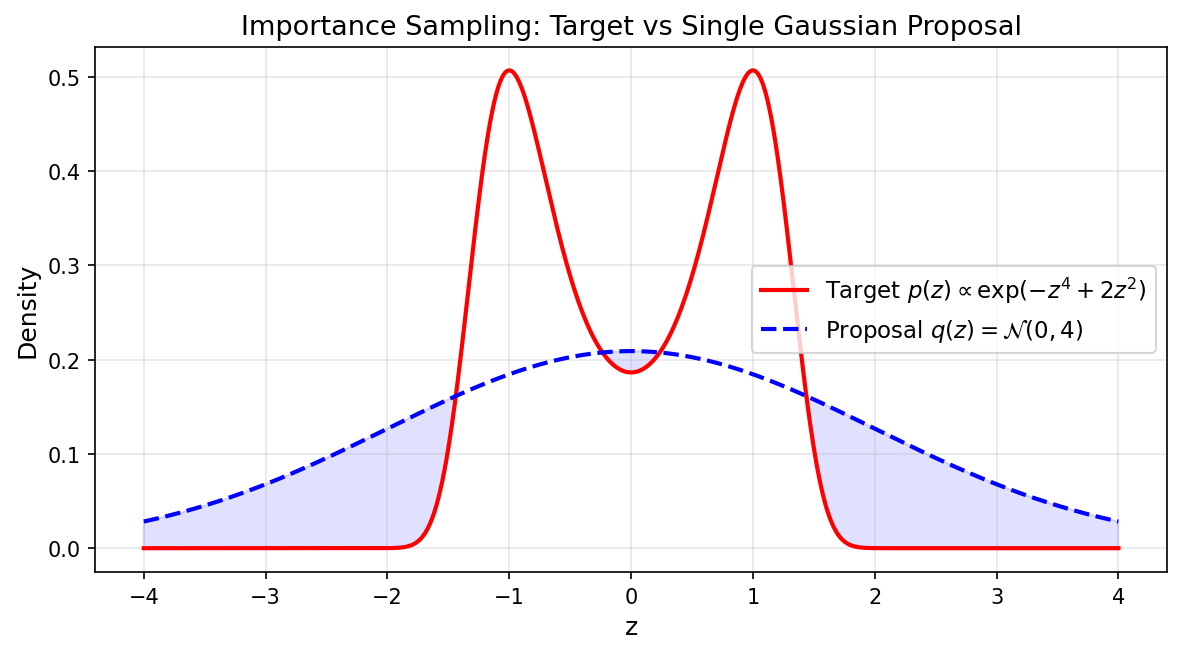
\includegraphics[width=0.92\textwidth]{images/is_single_gaussian_target_vs_proposal.png}
    \caption{Target density $p(z) \propto \exp(-z^4+2z^2)$
             versus the single Gaussian proposal
             $q(z)=\mathcal{N}(0,4)$.  The blue shaded region
             highlights where $q$ exceeds $p$ — wasted proposal
             mass.}
    \label{fig:is1_target}
\end{figure}

\subsubsection{Experiment~2: Gaussian Mixture Proposal}

\paragraph{Setup.}
To better match the bimodal target we replace the single Gaussian
with a two-component mixture:
\begin{equation}
    q(z) = \pi_1\,\mathcal{N}(z \mid \mu_1, \sigma_1^2)
         + \pi_2\,\mathcal{N}(z \mid \mu_2, \sigma_2^2)
    \label{eq:mixture_proposal}
\end{equation}

\begin{table}[H]
    \centering
    \begin{tabular}{lrl}
        \toprule
        \textbf{Parameter} & \textbf{Value} & \textbf{Purpose} \\
        \midrule
        $\pi_1, \pi_2$ & 0.5, 0.5 & Equal mixture weights \\
        $\mu_1, \mu_2$ & $-1.0,\; 1.0$ & Centres near the two modes \\
        $\sigma_1, \sigma_2$ & $0.5,\; 0.5$
            & Concentrate mass on each mode \\
        $L$ & 100{,}000 & Number of samples \\
        \bottomrule
    \end{tabular}
    \caption{Importance sampling setup --- mixture proposal.}
    \label{tab:is2_setup}
\end{table}

\begin{lstlisting}[caption={Importance sampling with a Gaussian mixture proposal.},
                   label=lst:is_mixture]
import numpy as np

def p_tilde(z):
    return np.exp(-z**4 + 2*z**2)

pi = np.array([0.5, 0.5])
mu = np.array([-1.0, 1.0])
sigma = np.array([0.5, 0.5])

def gaussian_pdf(z, mu, sigma):
    return (1 / (np.sqrt(2*np.pi) * sigma)) * \
           np.exp(-0.5 * ((z - mu) / sigma)**2)

def q_pdf(z):
    return (pi[0] * gaussian_pdf(z, mu[0], sigma[0]) +
            pi[1] * gaussian_pdf(z, mu[1], sigma[1]))

def sample_q(L):
    components = np.random.choice([0, 1], size=L, p=pi)
    z = np.zeros(L)
    for k in [0, 1]:
        idx = components == k
        z[idx] = np.random.normal(mu[k], sigma[k], np.sum(idx))
    return z

def f(z):
    return z**2

np.random.seed(42)
L = 100_000

z_samples = sample_q(L)
r_tilde = p_tilde(z_samples) / q_pdf(z_samples)
weights = r_tilde / np.sum(r_tilde)

E_f = np.sum(weights * f(z_samples))
print("Estimated E_p[z^2] =", E_f)
\end{lstlisting}

\begin{figure}[H]
    \centering
    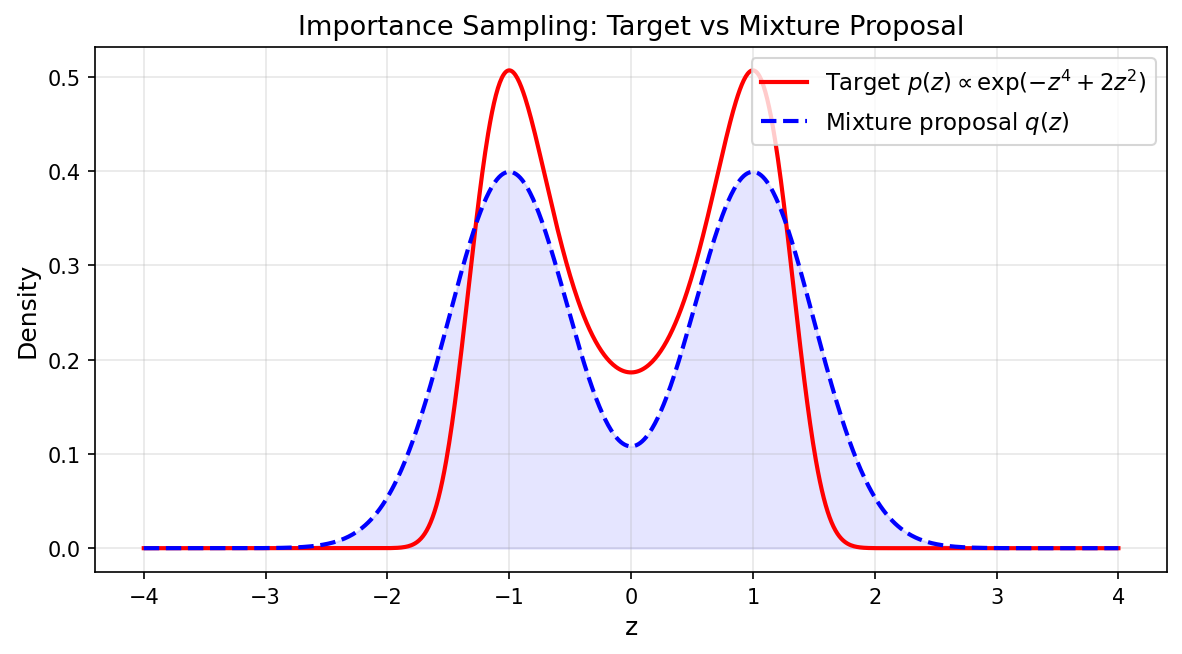
\includegraphics[width=0.92\textwidth]{images/is_mixture_target_vs_proposal.png}
    \caption{Target density versus the Gaussian mixture proposal.
             Each mixture component is centred on a target mode,
             yielding much better coverage than a single Gaussian.}
    \label{fig:is2_target}
\end{figure}

\subsubsection{Weight Distribution \& Effective Sample Size}

Figure~\ref{fig:is_weights} compares the importance-weight
distributions produced by the two proposals.

\begin{figure}[H]
    \centering
    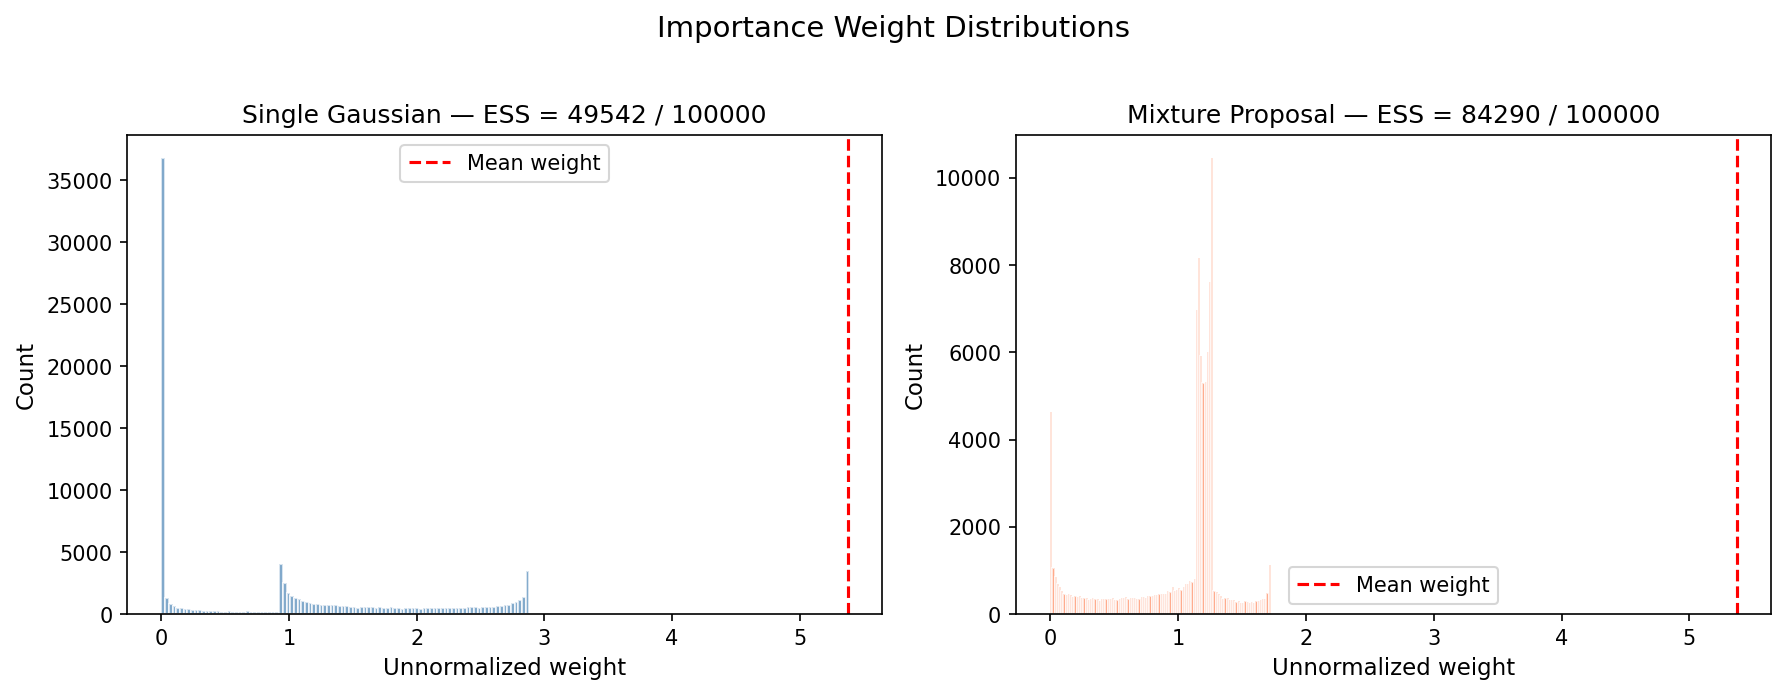
\includegraphics[width=\textwidth]{images/is_weight_comparison.png}
    \caption{Importance weight histograms.
             \textbf{Left:} Single Gaussian proposal
             (ESS~$\approx 49{,}542$).
             \textbf{Right:} Mixture proposal
             (ESS~$\approx 84{,}290$).
             The mixture's more uniform weights yield a
             substantially higher ESS.}
    \label{fig:is_weights}
\end{figure}

\subsubsection{Results}

\begin{table}[H]
    \centering
    \begin{tabular}{lrr}
        \toprule
        \textbf{Quantity}
            & \textbf{Single Gaussian}
            & \textbf{Mixture} \\
        \midrule
        $\hat{E}_p[z^2]$   & 0.8313 & 0.8325 \\
        ESS / $L$           & 49{,}542 / 100{,}000
                            & 84{,}290 / 100{,}000 \\
        \bottomrule
    \end{tabular}
    \caption{Importance sampling estimates and effective sample
             sizes for both proposals.}
    \label{tab:is_results}
\end{table}

Both proposals yield similar point estimates of
$\hat{E}_p[z^2] \approx 0.83$, but the mixture proposal achieves
an ESS that is $\approx 70\%$ higher, indicating much more uniform
weights and therefore a lower-variance estimator.

\subsubsection{Discussion}

\begin{itemize}
    \item \textbf{No wasted samples}: Unlike rejection sampling, every
          proposal contributes to the estimate — nothing is discarded.
    \item \textbf{Proposal design matters}: A poor proposal (e.g.\ a
          Gaussian far from the target modes) can produce a handful of
          samples with extreme weights that dominate the estimate,
          collapsing the ESS.
    \item \textbf{Self-normalization}: The normalized weights
          (Equation~\ref{eq:is_norm}) introduce a small bias of
          $O(1/L)$ but remove the need to know $Z_p$.
    \item \textbf{Curse of dimensionality}: In high dimensions the
          ratio $p/q$ varies exponentially, and the ESS can drop
          to~$\approx 1$.  Adaptive or sequential importance sampling
          (particle filters) mitigate this.
\end{itemize}

% ──────────────────────────────────────────────────────────
\subsection{Metropolis--Hastings Sampling}
\label{sec:mh}

Both rejection sampling and importance sampling require a
\emph{global} proposal that covers the entire support of the target.
As the dimensionality grows this becomes increasingly difficult.
\textbf{Metropolis--Hastings (MH)} sidesteps the problem by using a
\emph{local} proposal: at each step it proposes a small perturbation
of the current state and accepts or rejects it based on a simple
ratio test.  The resulting Markov chain has the target as its
stationary distribution.

\subsubsection{Algorithm}

Given an unnormalized target $\tilde{p}(z)$ and a symmetric proposal
kernel $q(z^* \mid z)$:

\begin{enumerate}
    \item Initialise $z_0$ (e.g.\ $z_0 = 0$).
    \item For $t = 1, 2, \ldots, T$:
    \begin{enumerate}
        \item \textbf{Propose}: draw
              $z^* \sim q(z^* \mid z_{t-1})$.
        \item \textbf{Acceptance ratio}:
              \begin{equation}
                  A \;=\; \min\!\left(1,\;
                  \frac{\tilde{p}(z^*)}{\tilde{p}(z_{t-1})}
                  \right)
                  \label{eq:mh_accept}
              \end{equation}
        \item With probability $A$ set $z_t = z^*$ (accept);
              otherwise $z_t = z_{t-1}$ (reject).
    \end{enumerate}
\end{enumerate}

Because only the \emph{ratio}
$\tilde{p}(z^*)/\tilde{p}(z_{t-1})$ appears, the normalizing
constant cancels and we only need the unnormalized target.

\paragraph{Detailed balance.}
The acceptance rule guarantees that the chain satisfies detailed
balance with respect to $p(z)$:
\begin{equation}
    p(z)\,q(z^* \mid z)\,A(z \to z^*)
    \;=\;
    p(z^*)\,q(z \mid z^*)\,A(z^* \to z)
    \label{eq:detailed_balance}
\end{equation}
which ensures $p(z)$ is the unique stationary distribution of the
chain (given mild ergodicity conditions).

\subsubsection{Experimental Setup}

\begin{table}[H]
    \centering
    \begin{tabular}{ll}
        \toprule
        \textbf{Component} & \textbf{Definition} \\
        \midrule
        Unnormalized target
            & $\tilde{p}(z) = \exp\!\bigl(-\tfrac{1}{8}z^4
              + \tfrac{3}{4}z^2 + 1\bigr)$ --- bimodal \\
        Proposal
            & Symmetric random walk:
              $z^* \sim \mathcal{N}(z_{t-1},\, 0.64)$
              (step size $\sigma = 0.8$) \\
        Chain length
            & $T = 20{,}000$ \\
        Burn-in
            & First $5{,}000$ samples discarded \\
        \bottomrule
    \end{tabular}
    \caption{Metropolis--Hastings experimental setup.}
    \label{tab:mh_setup}
\end{table}

\begin{lstlisting}[caption={Python implementation of the Metropolis--Hastings sampler.},
                   label=lst:mh]
import numpy as np

def p_tilde(z):
    return np.exp(-0.125 * z**4 + 0.75 * z**2 + 1)

def metropolis_sampler(p_tilde, n_samples=20000, step_size=0.8):
    samples = np.zeros(n_samples)
    z = 0.0  # initial state

    for i in range(n_samples):
        # Propose new point
        z_star = z + np.random.normal(0, step_size)

        # Acceptance probability
        acceptance_ratio = p_tilde(z_star) / p_tilde(z)
        A = min(1.0, acceptance_ratio)

        # Accept or reject
        if np.random.rand() < A:
            z = z_star

        samples[i] = z

    return samples

samples = metropolis_sampler(p_tilde)
\end{lstlisting}

The target density is bimodal with peaks near $z \approx \pm 1.7$.
The random-walk proposal is symmetric, so the acceptance ratio
reduces to the simple form in Equation~\ref{eq:mh_accept}.

\subsubsection{Samples vs.\ True Density}

Figure~\ref{fig:mh_hist} overlays the histogram of all $20{,}000$
samples with the numerically normalized target density.

\begin{figure}[H]
    \centering
    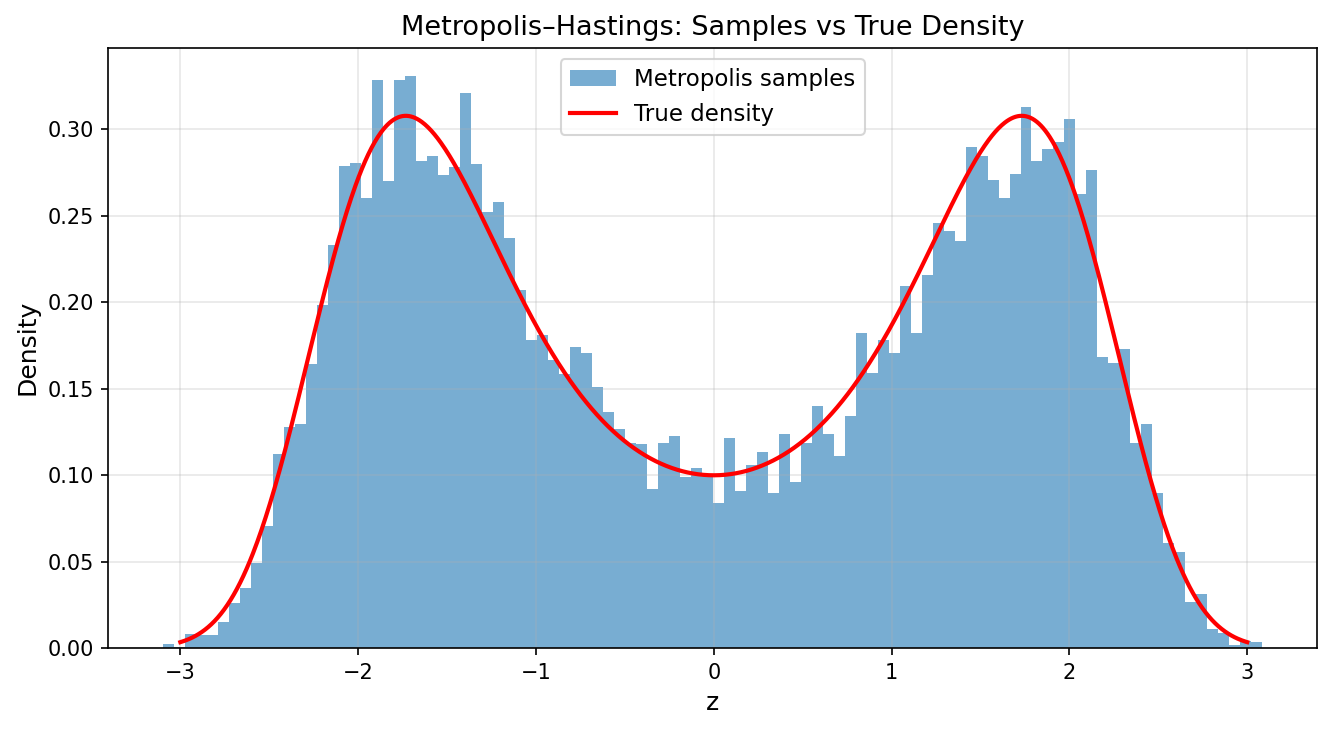
\includegraphics[width=0.92\textwidth]{images/mh_samples_vs_density.png}
    \caption{Histogram of $20{,}000$ Metropolis--Hastings samples
             versus the true target density
             $p(z) \propto \exp(-z^4/8 + 3z^2/4 + 1)$.
             Both modes are well-recovered.}
    \label{fig:mh_hist}
\end{figure}

\subsubsection{Trace Plot \& Convergence}

Figure~\ref{fig:mh_trace} shows two diagnostics:
\begin{itemize}
    \item \textbf{Left --- Trace plot}: the chain value $z_t$ over
          the first 2{,}000 iterations.  The chain mixes between the
          two modes, indicating adequate step size.
    \item \textbf{Right --- Running mean}: the cumulative average of
          $z_t^2$ (after burn-in) converges to the final estimate
          $\hat{E}[z^2]$.
\end{itemize}

\begin{figure}[H]
    \centering
    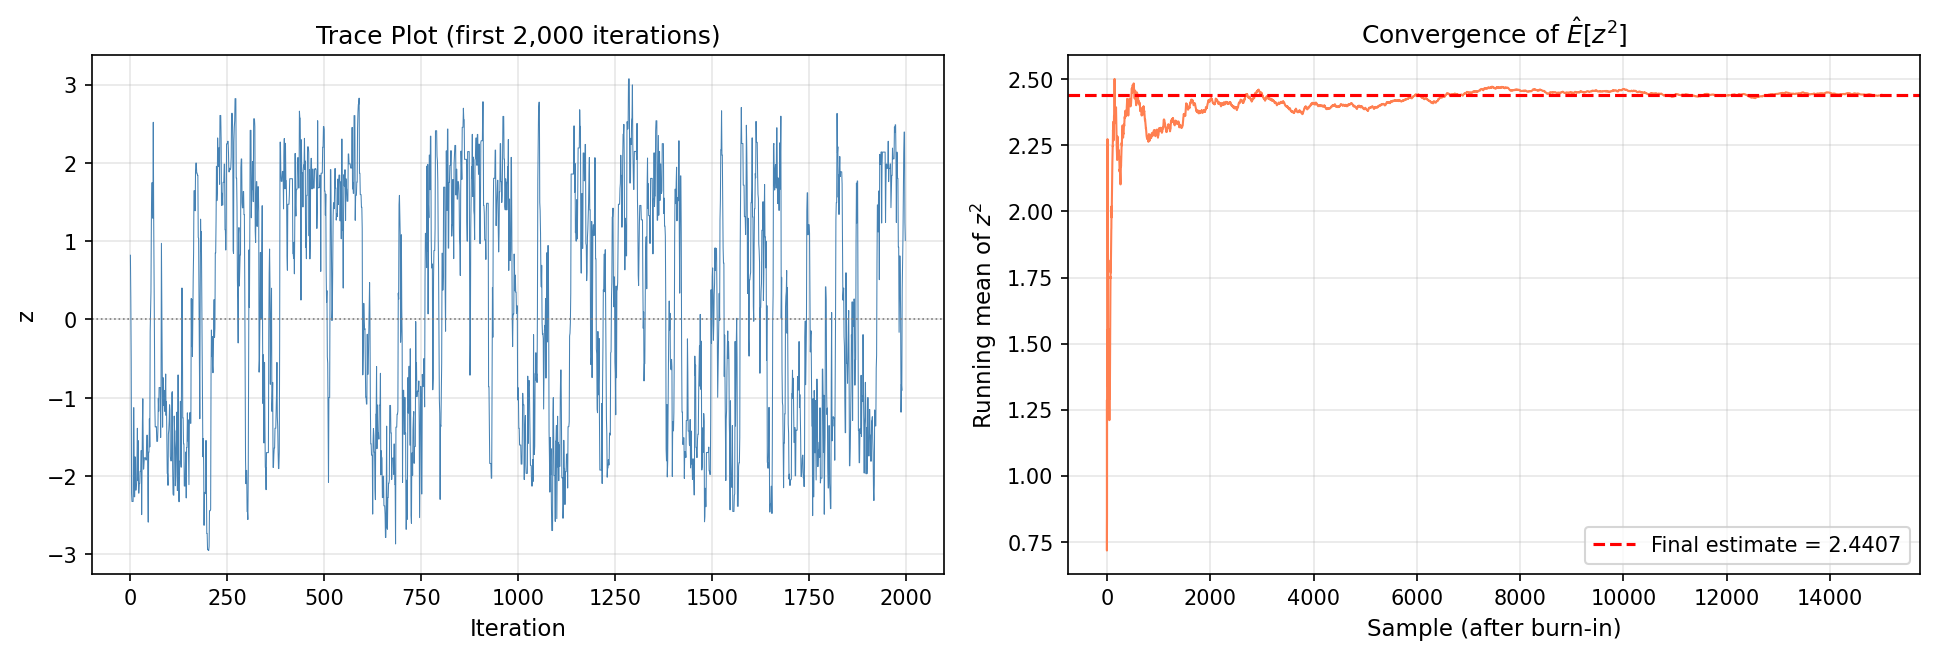
\includegraphics[width=\textwidth]{images/mh_trace_and_convergence.png}
    \caption{\textbf{Left:} Trace plot of the first 2{,}000
             iterations showing mode-hopping.
             \textbf{Right:} Running mean of $z^2$ after
             burn-in converging to
             $\hat{E}[z^2] \approx 2.44$.}
    \label{fig:mh_trace}
\end{figure}

\subsubsection{Results}

\begin{table}[H]
    \centering
    \begin{tabular}{lr}
        \toprule
        \textbf{Quantity} & \textbf{Value} \\
        \midrule
        Chain length $T$             & 20{,}000 \\
        Burn-in                      & 5{,}000 \\
        Acceptance rate               & $\approx 72.6\%$ \\
        $\hat{E}[z^2]$ (post burn-in) & 2.4407 \\
        \bottomrule
    \end{tabular}
    \caption{Metropolis--Hastings sampling statistics.}
    \label{tab:mh_results}
\end{table}

\subsubsection{Discussion}

\begin{itemize}
    \item \textbf{No envelope required}: Unlike rejection sampling,
          MH needs only a local proposal --- no global bounding
          constant $k$.
    \item \textbf{Acceptance rate}: The observed rate of
          $\approx 72.6\%$ is high, suggesting the step size could
          be increased slightly for faster exploration.  The
          theoretically optimal rate for a 1-D target is
          $\approx 44\%$.
    \item \textbf{Burn-in}: The first $5{,}000$ samples are
          discarded to remove the influence of the initial point.
    \item \textbf{Correlated samples}: Unlike importance sampling,
          MH samples are autocorrelated.  The effective number of
          independent samples is smaller than $T$.
    \item \textbf{Step-size trade-off}: Too small $\Rightarrow$
          high acceptance but slow mixing; too large $\Rightarrow$
          many rejections and the chain gets ``stuck.''
    \item \textbf{Scalability}: Random-walk MH scales
          poorly to high dimensions ($O(d)$ step-size tuning).
          Gradient-based variants such as \emph{MALA} or
          \emph{Hamiltonian Monte Carlo} are preferred in
          practice.
\end{itemize}

% ──────────────────────────────────────────────────────────
\subsection{Gibbs Sampling}
\label{sec:gibbs}

Metropolis--Hastings proposes moves in the \emph{full} state space
and then accepts or rejects.  When the state is multivariate,
designing a good joint proposal becomes difficult.
\textbf{Gibbs sampling} takes a fundamentally different approach:
it updates \textbf{one variable at a time}, drawing each variable
from its \emph{full conditional distribution} while keeping all
other variables fixed at their current values.

\subsubsection{Algorithm --- One Variable at a Time}

Consider a $d$-dimensional target
$p(z_1, z_2, \ldots, z_d)$.  Gibbs sampling proceeds as follows:

\begin{enumerate}
    \item Initialise $z_1^{(0)}, z_2^{(0)}, \ldots, z_d^{(0)}$.
    \item For $t = 1, 2, \ldots, T$, cycle through each dimension:
    \begin{align}
        z_1^{(t)} &\sim
            p\!\left(z_1 \;\middle|\;
            z_2^{(t-1)}, z_3^{(t-1)}, \ldots, z_d^{(t-1)}\right)
            \label{eq:gibbs_z1} \\
        z_2^{(t)} &\sim
            p\!\left(z_2 \;\middle|\;
            z_1^{(t)},\; z_3^{(t-1)}, \ldots, z_d^{(t-1)}\right)
            \label{eq:gibbs_z2} \\
        &\;\;\vdots \nonumber \\
        z_d^{(t)} &\sim
            p\!\left(z_d \;\middle|\;
            z_1^{(t)}, z_2^{(t)}, \ldots, z_{d-1}^{(t)}\right)
            \label{eq:gibbs_zd}
    \end{align}
\end{enumerate}

\noindent\textbf{Key property.}  Each step draws from the exact
\emph{conditional} distribution, so \textbf{every proposed value is
accepted} --- there is no accept/reject step and no tuning
parameters (step size, proposal width, etc.).

\paragraph{Connection to conditional distributions.}
The entire algorithm is driven by the conditionals
$p(z_i \mid \mathbf{z}_{\setminus i})$.  Gibbs sampling is
therefore applicable whenever:
\begin{enumerate}
    \item We can write down each conditional in closed form.
    \item We can \emph{sample} from each conditional efficiently.
\end{enumerate}
This is especially natural for \textbf{conjugate Bayesian models}
where every conditional belongs to a standard family (Gaussian,
Gamma, Dirichlet, etc.).

\paragraph{Why it converges.}
Each conditional-sampling sweep can be viewed as a special case of
Metropolis--Hastings with acceptance probability~1.  Therefore the
chain satisfies detailed balance with respect to the joint target,
and under mild conditions converges to $p(z_1, \ldots, z_d)$ as
$T \to \infty$.

\subsubsection{Experimental Setup: Correlated Bivariate Gaussian}

The target is a bivariate Gaussian with high correlation:
\begin{equation}
    \begin{pmatrix} z_1 \\ z_2 \end{pmatrix}
    \sim
    \mathcal{N}\!\left(
        \begin{pmatrix} 0 \\ 0 \end{pmatrix},\;
        \begin{pmatrix} 1 & \rho \\ \rho & 1 \end{pmatrix}
    \right),
    \qquad \rho = 0.9
    \label{eq:gibbs_target}
\end{equation}

The full conditionals are themselves Gaussians:
\begin{equation}
    z_1 \mid z_2 \;\sim\;
    \mathcal{N}\!\bigl(\rho\, z_2,\; 1-\rho^2\bigr),
    \qquad
    z_2 \mid z_1 \;\sim\;
    \mathcal{N}\!\bigl(\rho\, z_1,\; 1-\rho^2\bigr)
    \label{eq:gibbs_conditionals}
\end{equation}

This is an ideal setting for Gibbs: both conditionals are
standard Gaussians, so we can sample from them directly with
no approximation.

\begin{table}[H]
    \centering
    \begin{tabular}{lr}
        \toprule
        \textbf{Parameter} & \textbf{Value} \\
        \midrule
        Correlation $\rho$
            & 0.9 \\
        Conditional std $\sigma_{\text{cond}}
            = \sqrt{1-\rho^2}$
            & $\approx 0.436$ \\
        Total samples $T$
            & 10{,}000 \\
        Burn-in
            & 1{,}000 \\
        \bottomrule
    \end{tabular}
    \caption{Gibbs sampling experimental setup
             (bivariate Gaussian).}
    \label{tab:gibbs_setup}
\end{table}

\begin{lstlisting}[caption={Python implementation of Gibbs sampling for a bivariate Gaussian.},
                   label=lst:gibbs]
import numpy as np

rho = 0.9
sigma_cond = np.sqrt(1 - rho**2)
n_samples = 10000

z1 = np.zeros(n_samples)
z2 = np.zeros(n_samples)
z1[0], z2[0] = 0.0, 0.0

# Gibbs sampling loop
for t in range(1, n_samples):
    # Sample z1 | z2  (one variable at a time)
    z1[t] = np.random.normal(loc=rho * z2[t-1], scale=sigma_cond)

    # Sample z2 | z1  (use the UPDATED z1)
    z2[t] = np.random.normal(loc=rho * z1[t], scale=sigma_cond)
\end{lstlisting}

\subsubsection{Joint Scatter Plot}

Figure~\ref{fig:gibbs_scatter} shows the 9{,}000 post-burn-in
samples in the $(z_1, z_2)$ plane.  The elongated elliptical cloud
reflects the high positive correlation.

\begin{figure}[H]
    \centering
    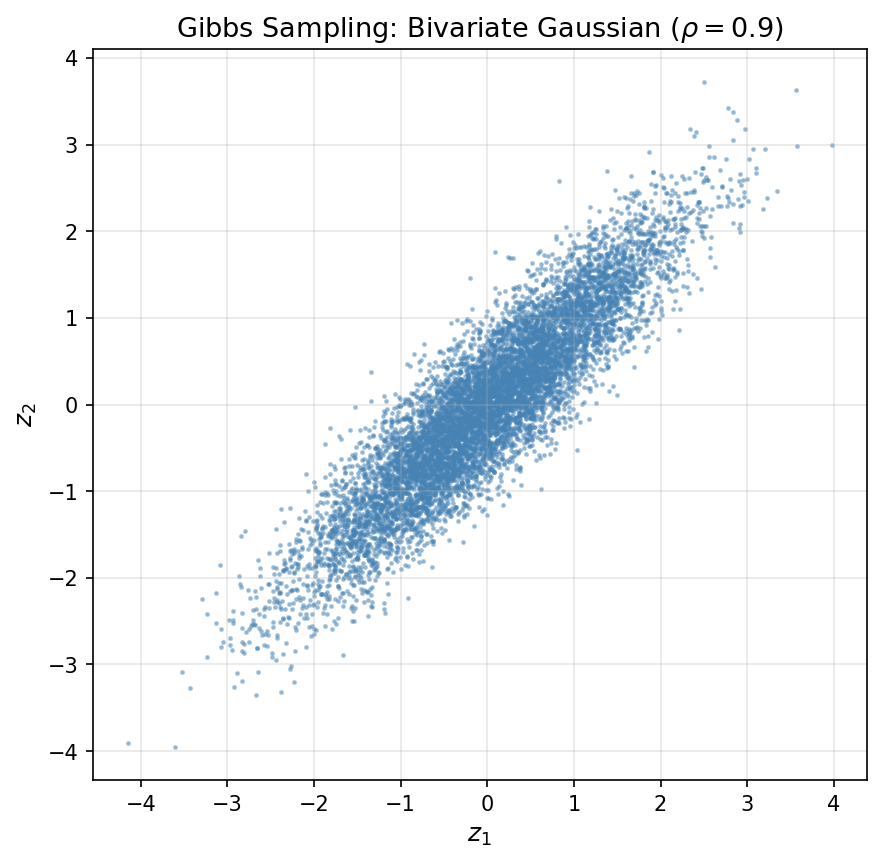
\includegraphics[width=0.65\textwidth]{images/gibbs_joint_scatter.png}
    \caption{Joint scatter plot of Gibbs samples from the bivariate
             Gaussian with $\rho = 0.9$.  The tilted elliptical
             shape matches the expected correlation structure.}
    \label{fig:gibbs_scatter}
\end{figure}

\subsubsection{Trace Plots \& Marginal Histograms}

Figure~\ref{fig:gibbs_traces} provides four diagnostics:
\begin{itemize}
    \item \textbf{Top row --- Trace plots} of $z_1$ and $z_2$
          over the first 500 iterations, illustrating the
          \emph{one-variable-at-a-time} updates: each coordinate
          oscillates while the other is momentarily held fixed.
    \item \textbf{Bottom row --- Marginal histograms} of $z_1$ and
          $z_2$ overlaid with the true $\mathcal{N}(0,1)$ marginal.
          The close match confirms correct sampling.
\end{itemize}

\begin{figure}[H]
    \centering
    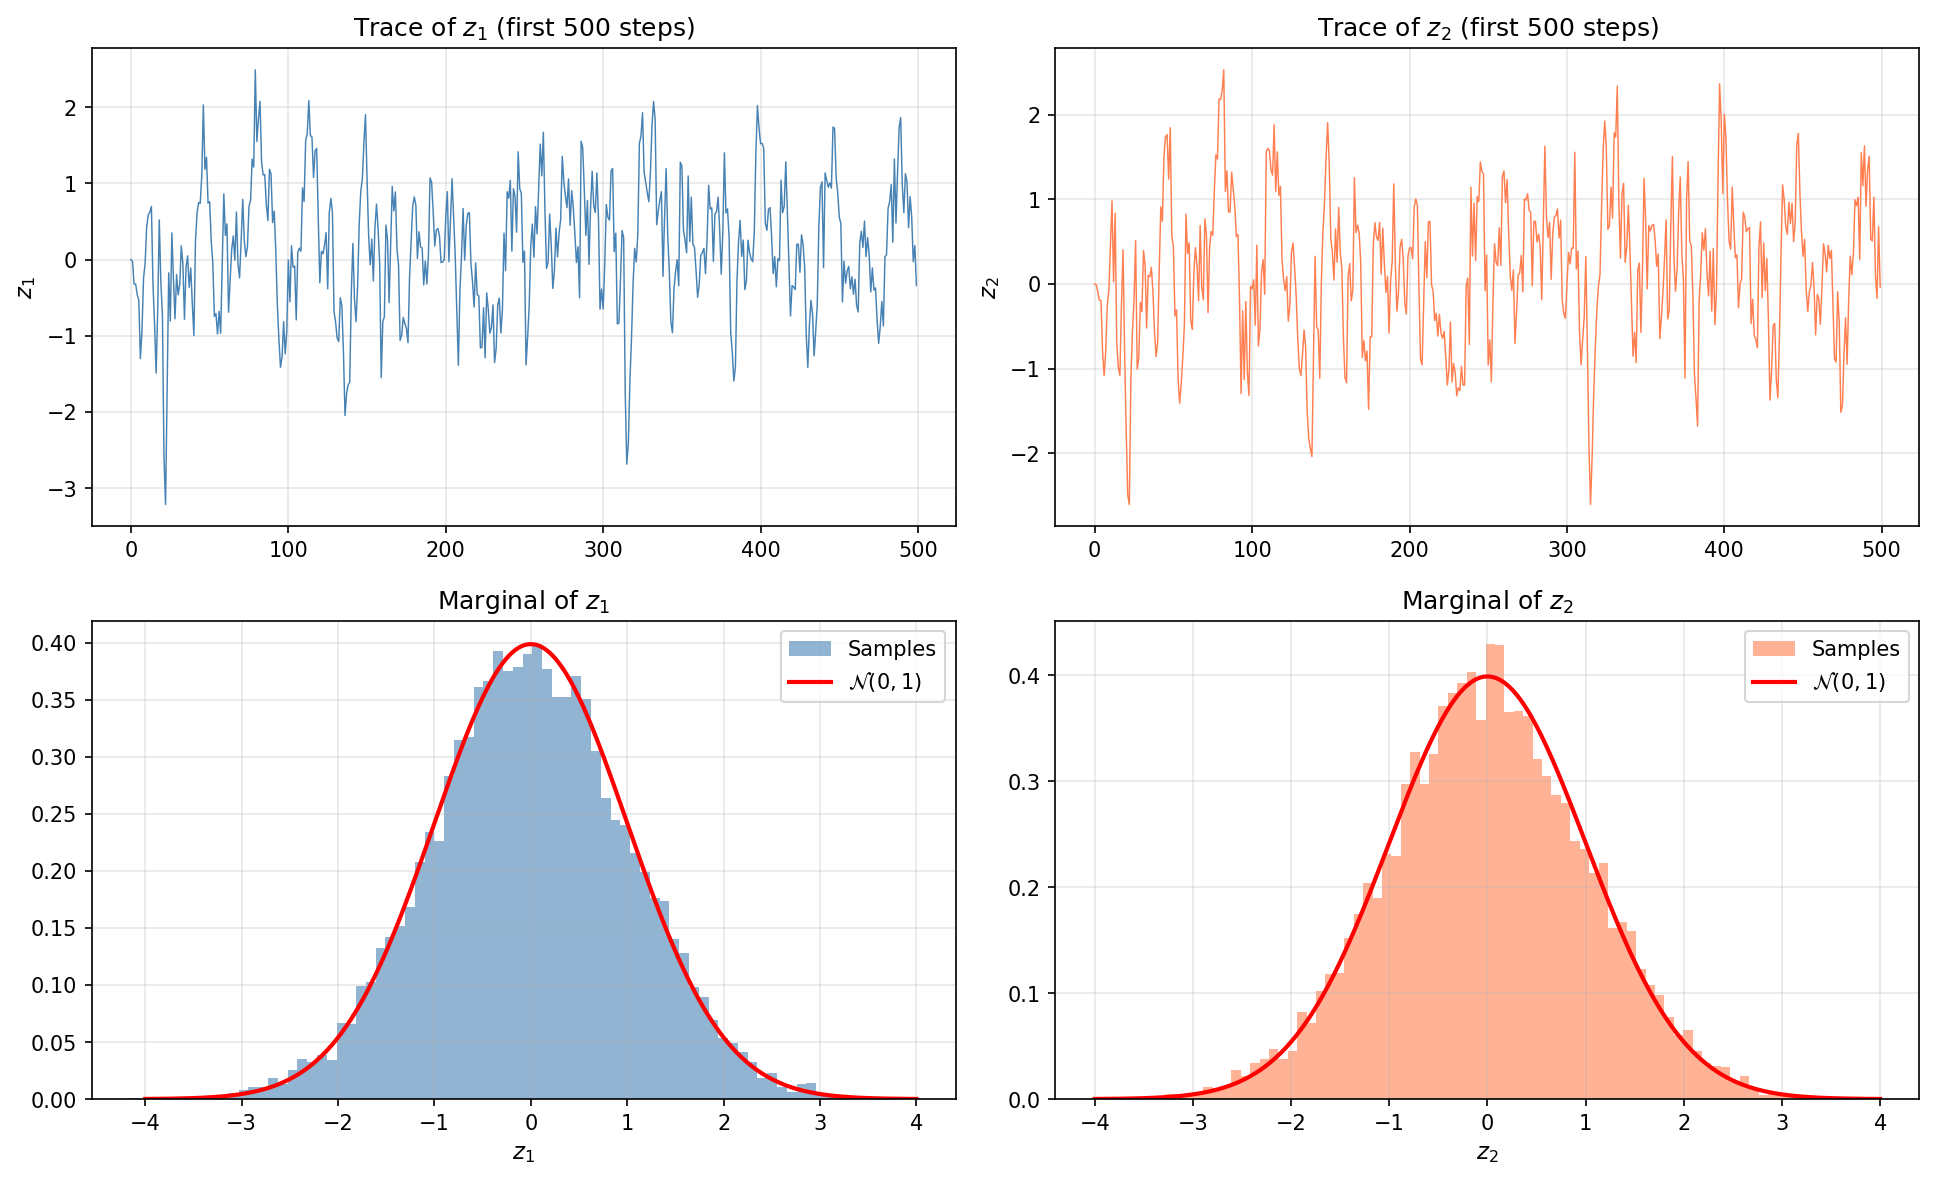
\includegraphics[width=\textwidth]{images/gibbs_traces_and_marginals.png}
    \caption{\textbf{Top:} Trace plots of $z_1$ (left) and $z_2$
             (right) showing the alternating conditional updates.
             \textbf{Bottom:} Marginal histograms versus the
             $\mathcal{N}(0,1)$ density (red).}
    \label{fig:gibbs_traces}
\end{figure}

\subsubsection{Results}

\begin{table}[H]
    \centering
    \begin{tabular}{lrr}
        \toprule
        \textbf{Statistic}
            & \textbf{Sample}
            & \textbf{True} \\
        \midrule
        Mean $z_1$        & $-0.004$  & 0 \\
        Mean $z_2$        & $-0.001$  & 0 \\
        Var $z_1$         & 1.053     & 1 \\
        Var $z_2$         & 1.049     & 1 \\
        Correlation        & 0.905     & 0.9 \\
        \bottomrule
    \end{tabular}
    \caption{Gibbs sampling: sample statistics versus true
             parameters of the bivariate Gaussian.}
    \label{tab:gibbs_results}
\end{table}

All sample statistics are close to the true values, confirming
that the Gibbs sampler has converged.

\subsubsection{Discussion}

\begin{itemize}
    \item \textbf{One variable at a time}: Gibbs avoids the
          difficult problem of designing a $d$-dimensional
          proposal.  Each update is a \emph{one-dimensional}
          draw from a known conditional, making implementation
          straightforward.
    \item \textbf{No tuning}: There is no step size, proposal
          width, or bounding constant to set --- the conditionals
          fully determine the updates.
    \item \textbf{100\% acceptance}: Every draw is exact, so no
          proposals are wasted.
    \item \textbf{Slow mixing under high correlation}: When
          $\rho \to 1$ the conditional variance
          $1 - \rho^2 \to 0$, so each update makes only a tiny
          step.  The chain explores the narrow ellipse slowly,
          requiring many more iterations to produce effectively
          independent samples.  Block or collapsed Gibbs
          variants can mitigate this.
    \item \textbf{Requires tractable conditionals}: If any
          conditional is unavailable in closed form, pure Gibbs
          cannot be used.  The \emph{Metropolis-within-Gibbs}
          hybrid (Section~\ref{sec:mwg}) replaces intractable
          conditionals with an MH step.
\end{itemize}

% ──────────────────────────────────────────────────────────
\subsection{Metropolis-within-Gibbs}
\label{sec:mwg}

\subsubsection{Why Is This Method Needed?}

We have already introduced two MCMC algorithms:
\begin{itemize}
    \item \textbf{Gibbs Sampling} (Section~\ref{sec:gibbs})
          cycles through each variable and draws from its
          \emph{full conditional} $p(z_i \mid \mathbf{z}_{\setminus i})$
          exactly.  It requires \emph{every} conditional to be
          available in closed form.
    \item \textbf{Metropolis--Hastings} (Section~\ref{sec:mh})
          proposes a \emph{joint} move from a proposal
          distribution $q(\mathbf{z}^* \mid \mathbf{z})$ and
          accepts or rejects.  It works for arbitrary targets
          but in high dimensions a single proposal must move all
          coordinates at once, which is hard to tune.
\end{itemize}

Many practical models---Bayesian neural networks, hierarchical
models, latent-variable models---have a mix of \emph{conjugate}
conditionals (easy to sample from) and \emph{non-conjugate}
conditionals (no closed-form density).  Neither pure Gibbs
nor pure MH is ideal:
\begin{itemize}
    \item Gibbs fails because at least one conditional is
          intractable.
    \item A \emph{joint} MH proposal in $d$ dimensions wastes
          effort: moves that improve one coordinate may worsen
          another, leading to low acceptance rates.
\end{itemize}

\textbf{Metropolis-within-Gibbs} combines the best of both
worlds.  It retains the Gibbs structure of updating
\emph{one variable at a time}, but replaces the exact
conditional draw with a \textbf{Metropolis--Hastings step}
for any variable whose conditional is intractable.
This gives three key advantages:
\begin{enumerate}
    \item \textbf{Tractable conditionals stay exact}: variables
          with closed-form conditionals are updated via Gibbs
          (100\% acceptance), preserving efficiency.
    \item \textbf{Intractable conditionals are handled}: a
          local MH proposal targets the intractable conditional
          directly, so the overall chain still converges to the
          correct joint distribution.
    \item \textbf{Lower-dimensional proposals}: because the MH
          step only proposes in the subspace of the intractable
          variable(s), the proposal is easier to tune and has a
          higher acceptance rate than a full-dimensional joint
          proposal.
\end{enumerate}

\subsubsection{Algorithm}

Given a joint target $p(z_1, z_2)$ where the conditional
$p(z_2 \mid z_1)$ is tractable but $p(z_1 \mid z_2)$ is not:

\begin{enumerate}
    \item \textbf{Gibbs step (exact)}: draw
          $z_2^{(t)} \sim p\!\left(z_2 \mid z_1^{(t-1)}\right)$
          --- a direct sample from the closed-form conditional.
    \item \textbf{Metropolis step (approximate)}: update
          $z_1$ using a random-walk proposal
          $z_1^* = z_1^{(t-1)} + \epsilon$,\;
          $\epsilon \sim \mathcal{N}(0, \sigma^2)$; accept
          with probability
          \[
              \alpha = \min\!\left(1,\;
                  \frac{p(z_1^*, z_2^{(t)})}
                       {p(z_1^{(t-1)}, z_2^{(t)})}\right).
          \]
          If rejected, keep $z_1^{(t)} = z_1^{(t-1)}$.
\end{enumerate}

Because the MH step targets the \emph{conditional}
$p(z_1 \mid z_2^{(t)})$ (a one-dimensional distribution), the
proposal scale $\sigma$ only needs to be tuned for a single
variable, not the entire joint space.

\subsubsection{Experimental Setup: Banana-Shaped Target}

The target density is defined via its log-probability:
\begin{equation}
    \log p(z_1, z_2) \;=\;
    -\tfrac{1}{2}\,z_1^{2}
    \;-\; \frac{(z_2 - z_1^{2})^{2}}{0.2}
    \label{eq:mwg_target}
\end{equation}

This produces a \textbf{banana-shaped} (non-Gaussian) density:
\begin{itemize}
    \item The conditional $z_2 \mid z_1$ is Gaussian:
          $\mathcal{N}(z_1^2,\, 0.1)$ --- \textbf{tractable},
          handled by a Gibbs step.
    \item The conditional $z_1 \mid z_2$ has no simple
          closed form --- \textbf{intractable}, handled by a
          Metropolis step.
\end{itemize}

This is precisely the scenario where neither pure Gibbs nor a
joint MH proposal would be ideal.  Pure Gibbs is impossible
(we cannot sample $z_1 \mid z_2$ exactly), and a joint MH
proposal would struggle with the strong nonlinear curvature
of the banana.

\begin{table}[H]
    \centering
    \begin{tabular}{lr}
        \toprule
        \textbf{Parameter} & \textbf{Value} \\
        \midrule
        Total samples $T$
            & 150{,}000 \\
        Burn-in
            & 5{,}000 \\
        MH proposal std $\sigma$
            & 0.3 \\
        \bottomrule
    \end{tabular}
    \caption{Metropolis-within-Gibbs experimental setup
             (banana-shaped target).}
    \label{tab:mwg_setup}
\end{table}

\begin{lstlisting}[caption={Python implementation of Metropolis-within-Gibbs for the banana-shaped target.},
                   label=lst:mwg]
import numpy as np

def log_p(z1, z2):
    return -0.5*z1**2 - 0.5*((z2 - z1**2)**2)/0.1

n_samples = 150000
z1 = np.zeros(n_samples)
z2 = np.zeros(n_samples)
z1[0], z2[0] = 0.0, 0.0

proposal_std = 0.3
n_accept = 0

for t in range(1, n_samples):
    # ---- Gibbs step for z2 | z1 (exact conditional)
    z2[t] = np.random.normal(z1[t-1]**2, np.sqrt(0.1))

    # ---- Metropolis step for z1 | z2 (intractable conditional)
    z1_prop = z1[t-1] + np.random.normal(0, proposal_std)
    log_alpha = log_p(z1_prop, z2[t]) - log_p(z1[t-1], z2[t])

    if np.log(np.random.rand()) < log_alpha:
        z1[t] = z1_prop
        n_accept += 1
    else:
        z1[t] = z1[t-1]
\end{lstlisting}

\subsubsection{Banana-Shaped Scatter Plot}

Figure~\ref{fig:mwg_scatter} shows the 145{,}000 post-burn-in
samples in the $(z_1, z_2)$ plane.  The characteristic
banana-shaped cloud confirms that the hybrid sampler successfully
explores the curved, non-Gaussian target.

\begin{figure}[H]
    \centering
    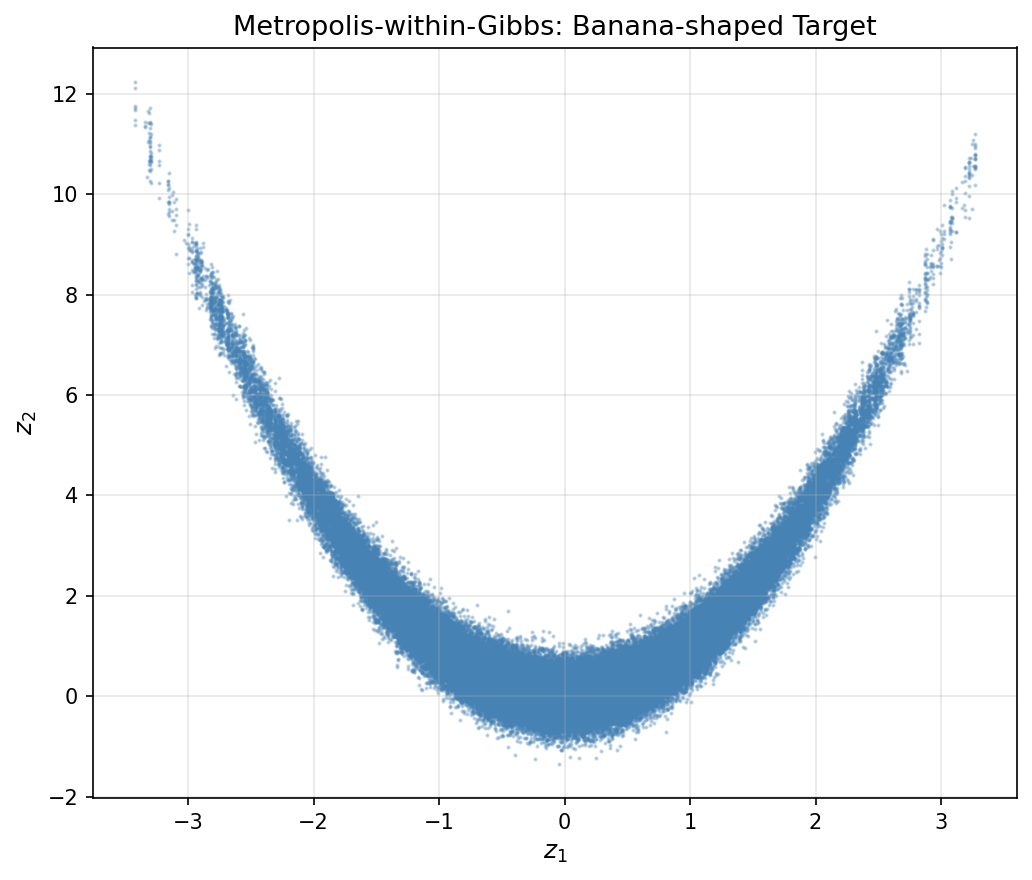
\includegraphics[width=0.70\textwidth]{images/mwg_banana_scatter.png}
    \caption{Metropolis-within-Gibbs samples from the
             banana-shaped target~\eqref{eq:mwg_target}.
             The nonlinear relationship $z_2 \approx z_1^{2}$
             is clearly visible.}
    \label{fig:mwg_scatter}
\end{figure}

\subsubsection{Trace Plots \& Marginal Histograms}

Figure~\ref{fig:mwg_traces} provides four diagnostics:
\begin{itemize}
    \item \textbf{Top-left --- $z_1$ trace} (Metropolis step):
          the random-walk character is visible --- the chain
          sometimes stays flat (rejected proposals) and
          sometimes jumps.
    \item \textbf{Top-right --- $z_2$ trace} (Gibbs step):
          larger jumps reflect the exact conditional draws,
          which can move freely given the current $z_1$.
    \item \textbf{Bottom row --- marginal histograms}: the
          $z_1$ marginal is approximately Gaussian while
          the $z_2$ marginal is right-skewed (since
          $z_2 \approx z_1^{2}$ adds positive bias).
\end{itemize}

\begin{figure}[H]
    \centering
    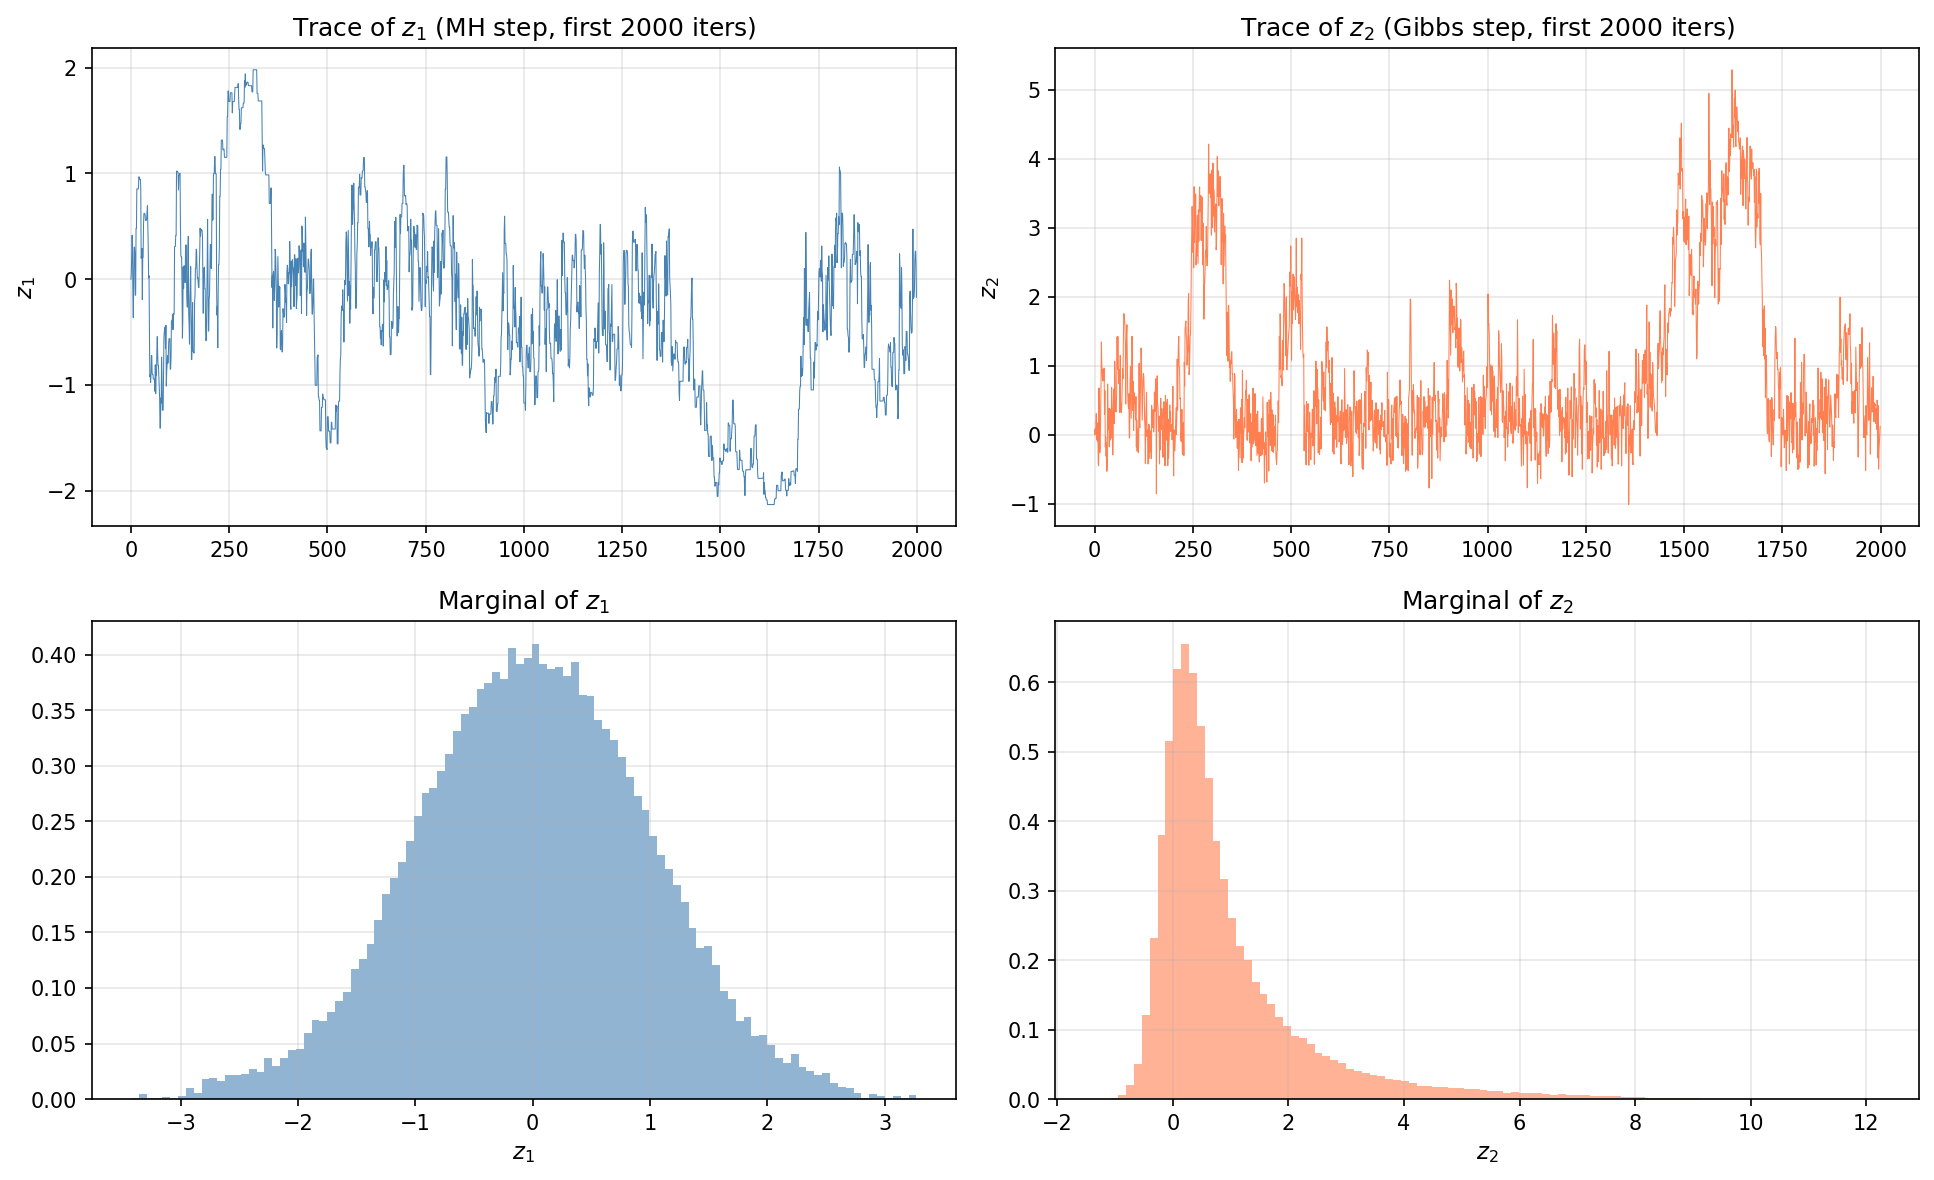
\includegraphics[width=\textwidth]{images/mwg_traces_and_marginals.png}
    \caption{\textbf{Top:} Trace plots of $z_1$ (MH step, left)
             and $z_2$ (Gibbs step, right) over 2{,}000
             iterations.  \textbf{Bottom:} Marginal histograms
             of $z_1$ and $z_2$ after burn-in.}
    \label{fig:mwg_traces}
\end{figure}

\subsubsection{Results}

\begin{table}[H]
    \centering
    \begin{tabular}{lr}
        \toprule
        \textbf{Statistic}
            & \textbf{Sample} \\
        \midrule
        MH acceptance rate ($z_1$ step)
            & 63.6\% \\
        Mean $z_1$
            & 0.002 \\
        Mean $z_2$
            & 0.974 \\
        Std $z_1$
            & 0.987 \\
        Std $z_2$
            & 1.404 \\
        \bottomrule
    \end{tabular}
    \caption{Metropolis-within-Gibbs: sample statistics for the
             banana-shaped target.}
    \label{tab:mwg_results}
\end{table}

The mean of $z_1$ is close to zero (the marginal is symmetric)
while $\mathrm{E}[z_2] \approx 1$ because
$z_2 \approx z_1^{2}$ and $\mathrm{E}[z_1^{2}] \approx 1$.
The acceptance rate of $\approx 64\%$ is in a good range,
indicating the proposal scale $\sigma = 0.3$ is well-tuned.

\subsubsection{Discussion}

\begin{itemize}
    \item \textbf{Hybrid strength}: The Gibbs update for $z_2$
          is exact (acceptance probability~1) while the MH
          update for $z_1$ adapts to the local conditional.
          This is more efficient than applying MH to both
          variables simultaneously.
    \item \textbf{Comparison with pure Methods}:
          \begin{itemize}
              \item \emph{Pure Gibbs} is impossible here because
                    $p(z_1 \mid z_2)$ has no closed form.
              \item \emph{Pure MH} with a 2D proposal would
                    struggle with the banana curvature;
                    Metropolis-within-Gibbs reduces the problem
                    to a well-behaved 1D conditional.
          \end{itemize}
    \item \textbf{When to use Metropolis-within-Gibbs}:
          whenever a model has a mixture of conjugate and
          non-conjugate conditionals --- common in hierarchical
          Bayesian models, mixture models with non-standard
          priors, and latent variable models.
    \item \textbf{Proposal tuning}: only the MH step requires
          tuning ($\sigma$).  Gibbs steps are automatic.
          Targeting an acceptance rate of $\sim 20$--$60\%$ for
          the MH components is a standard guideline.
    \item \textbf{Scalability}: in high-dimensional models with
          many intractable conditionals, each MH sub-step
          operates in a low-dimensional space, which is far
          easier than a single MH proposal in the full joint
          space.
\end{itemize}

% ──────────────────────────────────────────────────────────
\subsection{Ancestral Sampling}
\label{sec:ancestral}

\subsubsection{Bayesian Networks and Conditional Dependencies}

All the MCMC methods discussed so far---Metropolis--Hastings,
Gibbs, and Metropolis-within-Gibbs---draw \emph{correlated}
samples from a Markov chain and require a burn-in period before
the samples approximate the target distribution.  They are
designed for situations where we know the target density (or its
unnormalized form) but cannot sample from it directly.

\textbf{Ancestral sampling} addresses a fundamentally different
setting: the joint distribution is specified as a
\textbf{Bayesian network} (directed acyclic graph, DAG), and
\emph{every} conditional distribution $p(z_i \mid \mathrm{pa}(z_i))$
is available in closed form and easy to sample from.  In a Bayesian
network the joint factorizes according to the graph structure:
\begin{equation}
    p(z_1, z_2, \ldots, z_d)
    \;=\;
    \prod_{i=1}^{d}\, p\!\left(z_i \mid \mathrm{pa}(z_i)\right)
    \label{eq:bn_factorization}
\end{equation}
where $\mathrm{pa}(z_i)$ denotes the \emph{parents} of node $z_i$
in the DAG.  This factorization encodes \textbf{conditional
independence} relationships: each variable is conditionally
independent of its non-descendants given its parents.

Ancestral sampling exploits this structure directly.  By
traversing the nodes in \textbf{topological order} (parents
before children), each variable can be sampled from its
conditional distribution because all parent values are already
available.  The result is an \textbf{exact, independent} sample
from the full joint---no Markov chain, no burn-in, no
accept/reject step.

\subsubsection{Connection with Conditional Distributions}

The key insight linking ancestral sampling to the conditional
distributions used elsewhere in this document is:
\begin{itemize}
    \item In \textbf{Gibbs sampling}, we cycle through variables
          and sample each from its \emph{full conditional}
          $p(z_i \mid \mathbf{z}_{\setminus i})$, which
          conditions on \emph{all} other variables.
    \item In \textbf{Ancestral sampling}, we sample each
          variable from its \emph{local conditional}
          $p(z_i \mid \mathrm{pa}(z_i))$, which conditions
          only on the \emph{parent} variables.
\end{itemize}
Both methods rely on the ability to sample from conditional
distributions, but Gibbs requires the full conditionals (which
may be complicated), whereas ancestral sampling only requires
the \emph{local} conditionals dictated by the DAG---which are
typically the building blocks of the model itself.

\subsubsection{Algorithm}

Given a Bayesian network with $d$ nodes in topological order
$z_1, z_2, \ldots, z_d$:

\begin{enumerate}
    \item For $i = 1, 2, \ldots, d$:
    \begin{enumerate}
        \item Identify the parent values
              $\mathrm{pa}(z_i)$ (already sampled).
        \item Draw $z_i \sim p\!\left(z_i \mid \mathrm{pa}(z_i)\right)$.
    \end{enumerate}
    \item Return $(z_1, z_2, \ldots, z_d)$ as one \textbf{i.i.d.}\ sample
          from the joint.
\end{enumerate}

Repeating this $N$ times yields $N$ \textbf{independent} samples,
each drawn in $O(d)$ time.  There is no correlation between
successive samples and no burn-in is needed.

\subsubsection{Experimental Setup: Linear Gaussian Chain}

We consider a three-node chain
$z_1 \to z_2 \to z_3$:
\begin{equation}
    z_1 \sim \mathcal{N}(0,\, 1),\qquad
    z_2 \mid z_1 \sim \mathcal{N}(a\,z_1,\; \sigma^2),\qquad
    z_3 \mid z_2 \sim \mathcal{N}(b\,z_2,\; \tau^2)
    \label{eq:ancestral_chain}
\end{equation}

The DAG structure $z_1 \to z_2 \to z_3$ encodes the conditional
independence $z_3 \perp\!\!\perp z_1 \mid z_2$: given $z_2$,
knowing $z_1$ provides no additional information about $z_3$.
However, \emph{marginally} $z_1$ and $z_3$ are correlated
because $z_2$ mediates the dependence.

\begin{table}[H]
    \centering
    \begin{tabular}{lrl}
        \toprule
        \textbf{Parameter} & \textbf{Value}
            & \textbf{Meaning} \\
        \midrule
        $a$      & 1.5   & Slope $z_1 \to z_2$ \\
        $b$      & $-0.8$ & Slope $z_2 \to z_3$ \\
        $\sigma$ & 0.5   & Noise std for $z_2 \mid z_1$ \\
        $\tau$   & 0.3   & Noise std for $z_3 \mid z_2$ \\
        $N$      & 10{,}000 & Independent samples \\
        \bottomrule
    \end{tabular}
    \caption{Ancestral sampling experimental setup
             (linear Gaussian chain).}
    \label{tab:ancestral_setup}
\end{table}

Because the model is linear-Gaussian, the true marginals can be
computed analytically:
\begin{align}
    \mathrm{Var}(z_2) &= a^2 + \sigma^2 = 2.50,
        & \mathrm{Std}(z_2) &\approx 1.581 \nonumber\\
    \mathrm{Var}(z_3) &= b^2(a^2 + \sigma^2) + \tau^2 = 1.69,
        & \mathrm{Std}(z_3) &= 1.300
    \label{eq:ancestral_marginals}
\end{align}

\begin{lstlisting}[caption={Python implementation of ancestral sampling for a linear Gaussian chain.},
                   label=lst:ancestral]
import numpy as np

# Parameters for the chain: z1 -> z2 -> z3
a = 1.5       # slope z1 -> z2
b = -0.8      # slope z2 -> z3
sigma = 0.5   # noise std for z2 | z1
tau = 0.3     # noise std for z3 | z2

def ancestral_sample():
    z1 = np.random.normal(0, 1)             # p(z1)
    z2 = np.random.normal(a * z1, sigma)    # p(z2 | z1)
    z3 = np.random.normal(b * z2, tau)      # p(z3 | z2)
    return z1, z2, z3

N = 10000
samples = np.array([ancestral_sample() for _ in range(N)])
z1, z2, z3 = samples.T
\end{lstlisting}

\subsubsection{Pairwise Scatter Plots}

Figure~\ref{fig:ancestral_scatter} shows all three pairwise
relationships:
\begin{itemize}
    \item \textbf{Left ($z_1$ vs $z_2$)}: strong positive
          linear trend (slope $a=1.5$) --- a \emph{direct}
          dependency in the DAG.
    \item \textbf{Center ($z_2$ vs $z_3$)}: strong negative
          linear trend (slope $b=-0.8$) --- another \emph{direct}
          dependency.
    \item \textbf{Right ($z_1$ vs $z_3$)}: negative correlation
          even though there is no direct edge $z_1 \to z_3$ in
          the graph.  This is an \emph{indirect} (marginal)
          dependency mediated through $z_2$.
\end{itemize}

\begin{figure}[H]
    \centering
    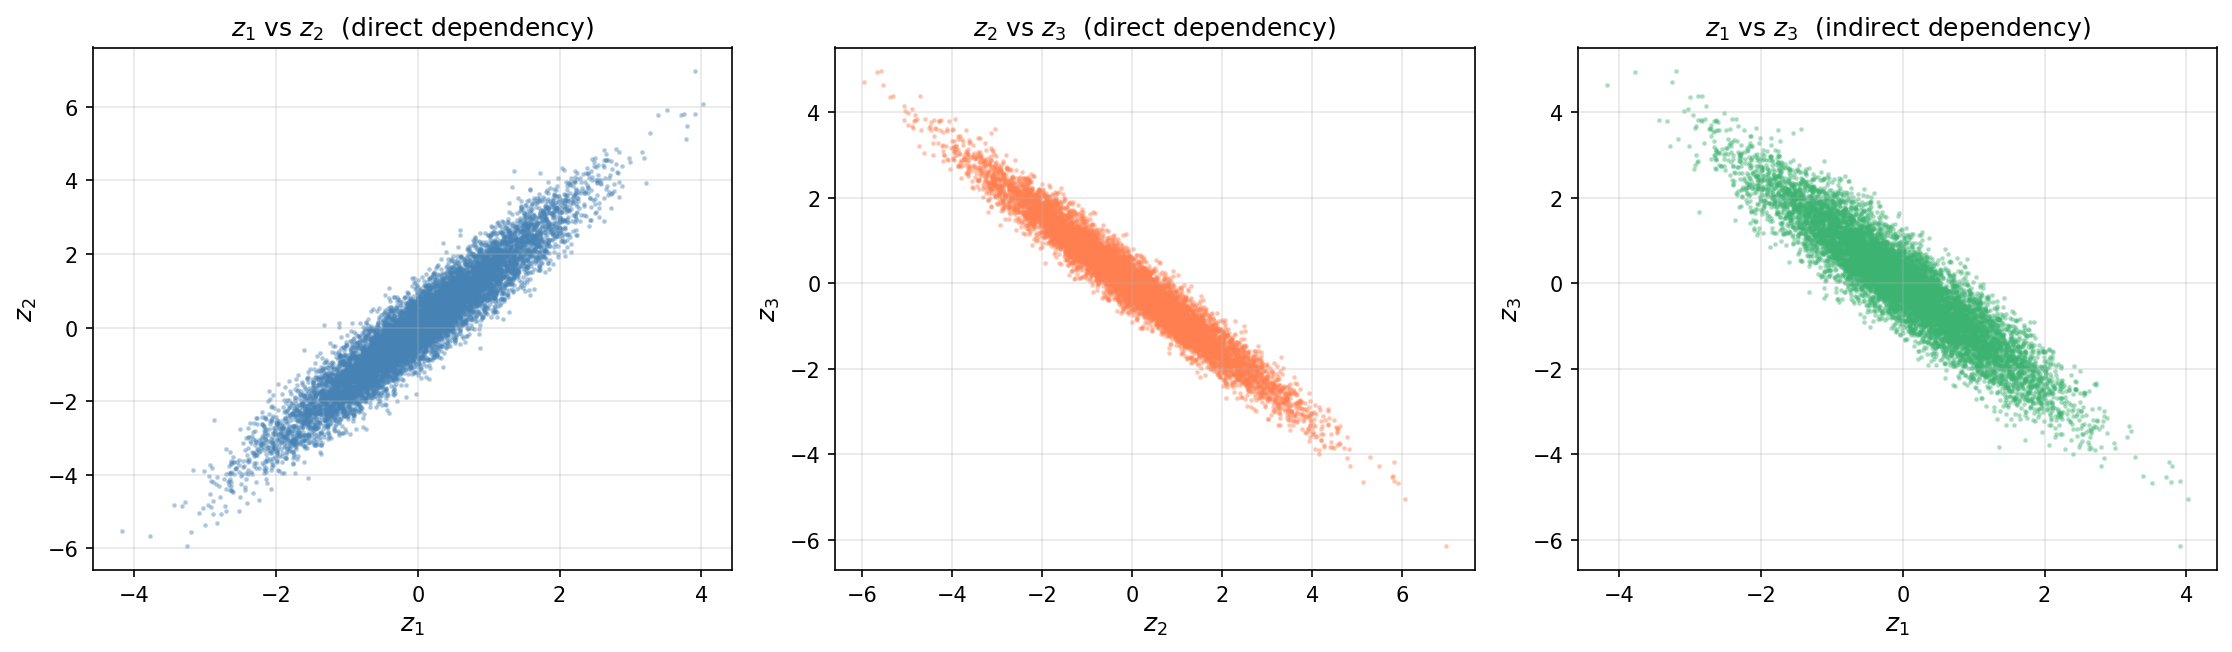
\includegraphics[width=\textwidth]{images/ancestral_pairwise_scatter.png}
    \caption{Pairwise scatter plots of 10{,}000 ancestral
             samples from the chain
             $z_1 \to z_2 \to z_3$.  Direct dependencies
             (left, center) are clearly linear; the indirect
             dependency (right) arises through $z_2$.}
    \label{fig:ancestral_scatter}
\end{figure}

\subsubsection{Marginal Histograms}

Figure~\ref{fig:ancestral_marginals} overlays the sample
histograms with the true Gaussian marginal densities.  All
three agree closely, confirming that ancestral sampling
produces exact samples from the joint.

\begin{figure}[H]
    \centering
    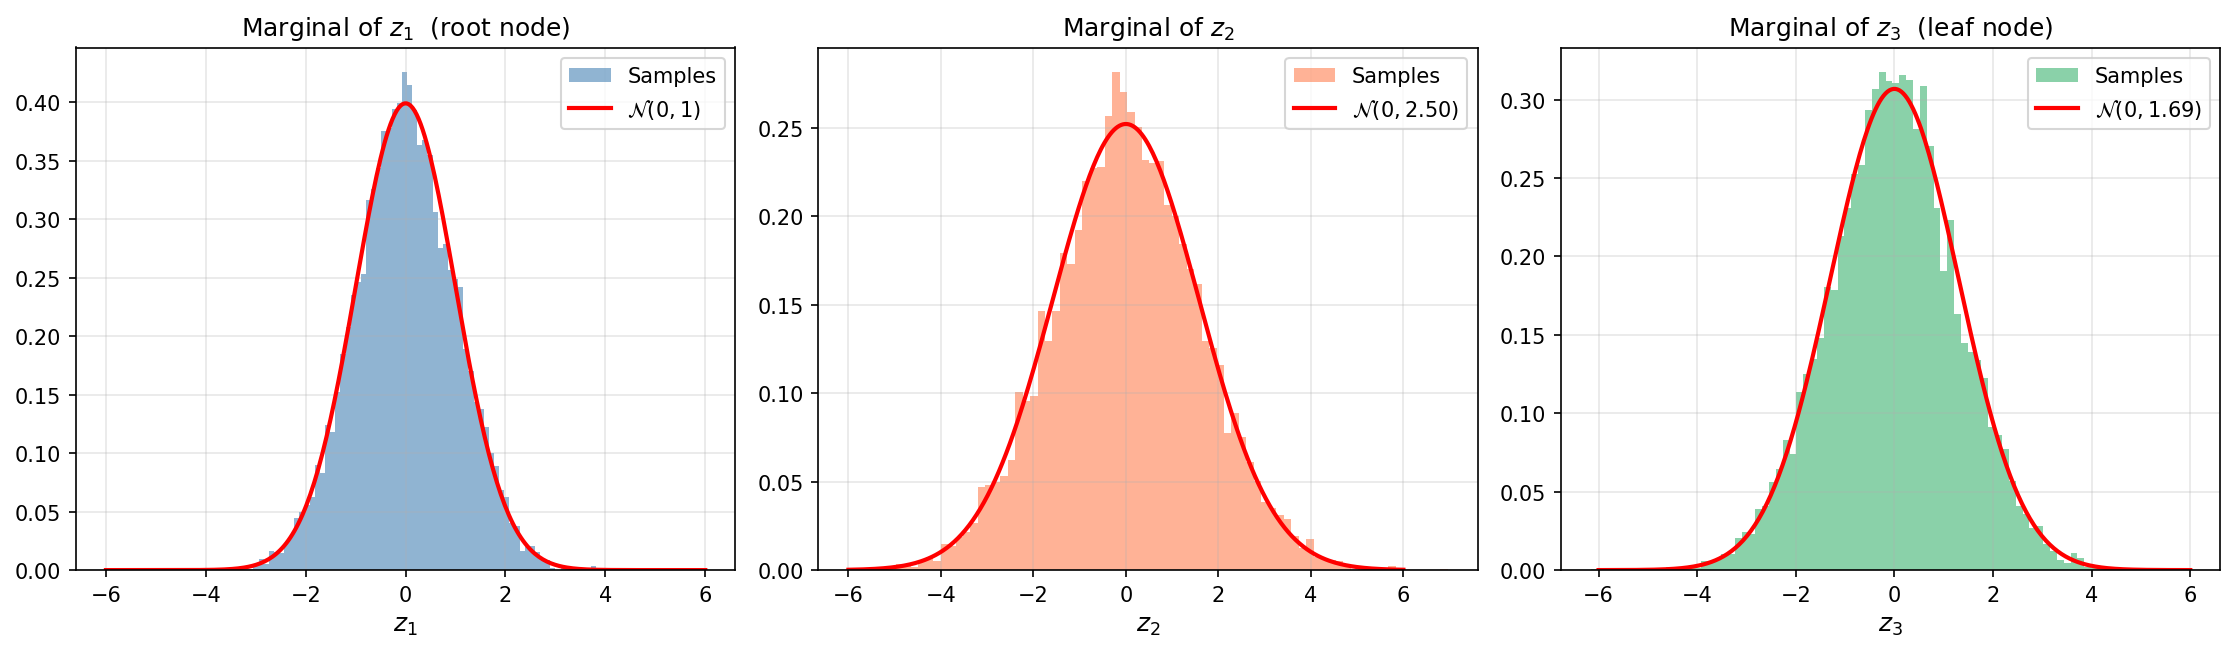
\includegraphics[width=\textwidth]{images/ancestral_marginal_histograms.png}
    \caption{Marginal histograms of $z_1$ (root), $z_2$, and
             $z_3$ (leaf) overlaid with the true Gaussian
             densities (red).  Labels indicate the node's
             role in the DAG.}
    \label{fig:ancestral_marginals}
\end{figure}

\subsubsection{Results}

\begin{table}[H]
    \centering
    \begin{tabular}{lrr}
        \toprule
        \textbf{Statistic}
            & \textbf{Sample}
            & \textbf{True} \\
        \midrule
        Mean $z_1$         & 0.012   & 0 \\
        Mean $z_2$         & 0.021   & 0 \\
        Mean $z_3$         & $-0.018$ & 0 \\
        Std $z_1$          & 1.007   & 1.000 \\
        Std $z_2$          & 1.589   & 1.581 \\
        Std $z_3$          & 1.303   & 1.300 \\
        Corr($z_1, z_2$)   & 0.949   & $a/\mathrm{Std}(z_2) \approx 0.949$ \\
        Corr($z_2, z_3$)   & $-0.974$ & $b\,\mathrm{Std}(z_2)/\mathrm{Std}(z_3) \approx -0.973$ \\
        Corr($z_1, z_3$)   & $-0.924$ & $ab/\mathrm{Std}(z_3) \approx -0.923$ \\
        \bottomrule
    \end{tabular}
    \caption{Ancestral sampling: sample statistics versus
             analytically computed true values.}
    \label{tab:ancestral_results}
\end{table}

All sample statistics match the analytical values to within
Monte Carlo noise, confirming that the sampler is exact.

\subsubsection{Discussion}

\begin{itemize}
    \item \textbf{Bayesian network structure}: Ancestral
          sampling directly mirrors the DAG factorization
          \eqref{eq:bn_factorization}.  Each node is sampled
          from its \emph{local conditional}
          $p(z_i \mid \mathrm{pa}(z_i))$, which is typically
          the model specification itself---no additional
          derivation is required.
    \item \textbf{Conditional independence in action}:
          the chain structure $z_1 \to z_2 \to z_3$ implies
          $z_3 \perp\!\!\perp z_1 \mid z_2$.  Yet the
          scatter plot of $(z_1, z_3)$ shows strong marginal
          correlation, illustrating how conditional independence
          does \emph{not} imply marginal independence.
    \item \textbf{Exact and i.i.d.}: Unlike MCMC methods,
          every sample is independent.  There is no burn-in,
          no autocorrelation, and no convergence diagnostics
          to worry about.  The effective sample size equals
          the actual sample size.
    \item \textbf{Comparison with MCMC}:
          \begin{itemize}
              \item \emph{Gibbs / MH / MwG} are needed when we
                    cannot sample from the conditionals
                    directly, or when we must condition on
                    observed evidence (posterior inference).
              \item \emph{Ancestral sampling} is only possible
                    when the model is a DAG and all local
                    conditionals are tractable---the
                    ``forward'' or ``generative'' direction.
          \end{itemize}
    \item \textbf{Limitation --- no conditioning on evidence}:
          Ancestral sampling draws from the \emph{prior}
          (or joint).  If we observe $z_3 = z_3^{\text{obs}}$
          and want to sample from
          $p(z_1, z_2 \mid z_3 = z_3^{\text{obs}})$, ancestral
          sampling cannot help directly---we would need
          likelihood weighting, MCMC, or variational methods.
    \item \textbf{Scalability}: for deep generative models
          (e.g., variational autoencoders, diffusion models),
          ancestral sampling is the standard way to generate
          new data by forwarding through the learned
          conditional distributions.
\end{itemize}

% ──────────────────────────────────────────────────────────
\subsection{Langevin Dynamics}
\label{sec:langevin}

\subsubsection{From Gradient Descent to Sampling}

Consider the task of \emph{minimizing} an energy function $E(x)$.
The standard \textbf{gradient descent} update is
\begin{equation}
    x_{t+1} \;=\; x_t \;-\; \eta\,\nabla E(x_t)
    \label{eq:gd_update}
\end{equation}
where $\eta > 0$ is the step size (learning rate).  This
deterministic rule drives $x$ toward the \emph{nearest} local
minimum of $E$ and stays there forever.

Now suppose we don't just want the mode---we want to
\textbf{sample} from the full distribution
$p(x) \propto \exp\!\bigl(-E(x)\bigr)$.
Langevin dynamics achieves this by adding
\textbf{calibrated Gaussian noise} to the gradient step:
\begin{equation}
    \boxed{\;
    x_{t+1} \;=\; x_t \;-\;
    \eta\,\nabla E(x_t)
    \;+\; \sqrt{2\eta}\;\xi_t,
    \qquad \xi_t \sim \mathcal{N}(0,1)
    \;}
    \label{eq:langevin_update}
\end{equation}

The two terms play complementary roles:
\begin{itemize}
    \item \textbf{Gradient drift}
          $-\eta\,\nabla E(x_t)$:
          deterministic force that pushes $x$ toward
          high-probability (low-energy) regions---exactly
          the same as gradient descent.
    \item \textbf{Noise injection}
          $\sqrt{2\eta}\;\xi_t$:
          stochastic perturbation that prevents the chain
          from collapsing onto a single mode.  The specific
          scaling $\sqrt{2\eta}$ ensures that the stationary
          distribution of the continuous-time process is
          exactly $p(x)$.
\end{itemize}

\paragraph{Key difference from gradient descent.}
Gradient descent converges to \emph{one} minimum.
Langevin dynamics explores \emph{the entire distribution},
visiting all modes with probability proportional to their
density.  The noise turns an \emph{optimizer} into a
\emph{sampler}.

\subsubsection{The Energy Function and the Score Function}

\paragraph{Energy function.}
The \textbf{energy function} (or negative log-likelihood)
$E(x)$ maps each state to a scalar ``energy.'' Low energy
corresponds to high probability:
\begin{equation}
    p(x) \;=\; \frac{1}{Z}\,\exp\!\bigl(-E(x)\bigr),
    \qquad
    Z = \int \exp\!\bigl(-E(x)\bigr)\,dx
    \label{eq:boltzmann}
\end{equation}
This is the \textbf{Boltzmann distribution} from statistical
physics.  Sampling from $p(x)$ is equivalent to exploring the
energy landscape $E(x)$.

\paragraph{Score function.}
The \textbf{score function} is the gradient of the
log-density:
\begin{equation}
    \nabla_x \log p(x)
    \;=\; -\nabla_x E(x)
    \label{eq:score}
\end{equation}
Note that the normalizing constant $Z$ disappears after
taking the gradient of the log---this is why Langevin dynamics
needs only the \emph{unnormalized} density, just like
Metropolis--Hastings.

The Langevin update~\eqref{eq:langevin_update} can
therefore be rewritten in terms of the score:
\begin{equation}
    x_{t+1} \;=\; x_t
    \;+\; \eta\,\nabla_x \log p(x_t)
    \;+\; \sqrt{2\eta}\;\xi_t
    \label{eq:langevin_score}
\end{equation}
The chain drifts in the direction of \emph{increasing}
log-probability (i.e.\@ toward high-density regions) and
fluctuates around them due to the noise.

\subsubsection{Energy Function $\leftrightarrow$ Probability
               Distribution}
\label{sec:energy_prob}

The relationship $p(x) = Z^{-1}\exp(-E(x))$ is a powerful
bijection between energy landscapes and probability
distributions.  It has several important consequences:

\begin{enumerate}
    \item \textbf{Minima of $E(x)$ $\,\Longleftrightarrow\,$
          modes of $p(x)$}.
          Every local minimum of the energy is a local
          maximum (mode) of the density.  A deeper energy
          well corresponds to a taller, more probable mode.

    \item \textbf{Curvature of $E(x)$ $\,\Longleftrightarrow\,$
          concentration of $p(x)$}.
          A narrow energy well (high second derivative)
          produces a sharp, concentrated peak in $p(x)$;
          a broad well produces a wide, diffuse mode.
          Formally, for a quadratic energy
          $E(x) = \tfrac{1}{2}\lambda\,x^2$, the resulting
          distribution is
          $\mathcal{N}(0, \lambda^{-1})$.

    \item \textbf{Energy barriers $\,\Longleftrightarrow\,$
          low-probability valleys}.
          An energy barrier (local maximum of $E$) between
          two minima corresponds to a region of
          \emph{very low probability} separating two modes.
          The sampler must cross this barrier to hop between
          modes, which requires the noise to overcome the
          energy difference---this is why multi-modal sampling
          can be slow.

    \item \textbf{Flat energy $\,\Longleftrightarrow\,$
          uniform distribution}.
          If $E(x) = \text{const}$, then $p(x)$ is uniform---no
          region is preferred.

    \item \textbf{Universality}.
          \emph{Any} probability distribution on a continuous
          space can be written in Boltzmann form: simply define
          $E(x) = -\log \tilde{p}(x)$ for any unnormalized
          density $\tilde{p}$.  This makes the energy--probability
          connection fully general, not limited to physics
          applications.
\end{enumerate}

\paragraph{Caveat: continuous densities only.}
The Boltzmann form $p(x) \propto \exp(-E(x))$ and the Langevin
update require the state space to be \emph{continuous} and $E(x)$
to be \emph{differentiable}.  For \textbf{discrete distributions}
(probability mass functions), $\nabla E$ is undefined and Langevin
dynamics cannot be applied directly.  Discrete targets require
discrete MCMC methods (e.g., Gibbs sampling with discrete
conditionals, or discrete Metropolis--Hastings proposals).

\subsubsection{Connection with Gradient Descent}

Table~\ref{tab:gd_vs_langevin} summarizes the relationship
between gradient descent and Langevin dynamics:

\begin{table}[H]
    \centering
    \begin{tabular}{lcc}
        \toprule
            & \textbf{Gradient Descent}
            & \textbf{Langevin Dynamics} \\
        \midrule
        \textbf{Update}
            & $x_{t+1} = x_t - \eta\,\nabla E$
            & $x_{t+1} = x_t - \eta\,\nabla E + \sqrt{2\eta}\,\xi$ \\
        \textbf{Goal}
            & Find $\arg\min_x E(x)$
            & Sample from $p(x) \propto e^{-E(x)}$ \\
        \textbf{Noise}
            & None (deterministic)
            & Gaussian, $\xi \sim \mathcal{N}(0,1)$ \\
        \textbf{Output}
            & Single point (one mode)
            & Distribution of samples (all modes) \\
        \textbf{Convergence}
            & To nearest minimum
            & To stationary distribution $p(x)$ \\
        \textbf{Multi-modal}
            & Trapped in one basin
            & Can hop between modes (given enough time) \\
        \bottomrule
    \end{tabular}
    \caption{Gradient descent vs.\ Langevin dynamics:
             adding calibrated noise transforms an optimizer
             into a sampler.}
    \label{tab:gd_vs_langevin}
\end{table}

\subsubsection{Experimental Setup: Double-Well Potential}

The target is defined via a quartic energy with two minima:
\begin{equation}
    E(x) = \tfrac{1}{4}\,x^{4} - \tfrac{1}{2}\,x^{2},
    \qquad
    \nabla E(x) = x^{3} - x
    \label{eq:double_well}
\end{equation}

The energy has:
\begin{itemize}
    \item Two \textbf{minima} at $x = \pm 1$ (where
          $\nabla E = 0$ and $\nabla^2 E > 0$), corresponding
          to the two \textbf{modes} of $p(x)$.
    \item An \textbf{energy barrier} at $x = 0$ (a local
          maximum of $E$), corresponding to a
          \textbf{low-probability valley} between the modes.
\end{itemize}

\begin{table}[H]
    \centering
    \begin{tabular}{lrl}
        \toprule
        \textbf{Parameter} & \textbf{Value}
            & \textbf{Purpose} \\
        \midrule
        Step size $\eta$
            & 0.04  & Discretization granularity \\
        Chain length $T$
            & 500{,}000 & Total iterations \\
        Initial point $x_0$
            & 3.0   & Far from both modes \\
        Burn-in
            & 1{,}000 & Samples discarded \\
        \bottomrule
    \end{tabular}
    \caption{Langevin dynamics experimental setup
             (double-well potential).}
    \label{tab:langevin_setup}
\end{table}

\begin{lstlisting}[caption={Python implementation of Langevin dynamics for the double-well potential.},
                   label=lst:langevin]
import numpy as np

def energy(x):
    return 0.25*x**4 - 0.5*x**2  # double-well potential

def grad_energy(x):
    return x**3 - x               # gradient of E(x)

eta = 0.04       # step size
T = 500000       # total iterations
x = 3.0          # initial point (far from modes)
burn_in = 1000

samples = np.zeros(T)
for t in range(T):
    noise = np.sqrt(2*eta) * np.random.randn()
    x = x - eta * grad_energy(x) + noise
    samples[t] = x
\end{lstlisting}

\subsubsection{Energy Landscape \& Target Density}

Figure~\ref{fig:langevin_energy} shows the energy function
and the corresponding target density side by side.  The
two minima of $E$ at $x = \pm 1$ become the two modes of
$p(x)$, and the energy barrier at $x = 0$ becomes the
low-probability valley between them.

\begin{figure}[H]
    \centering
    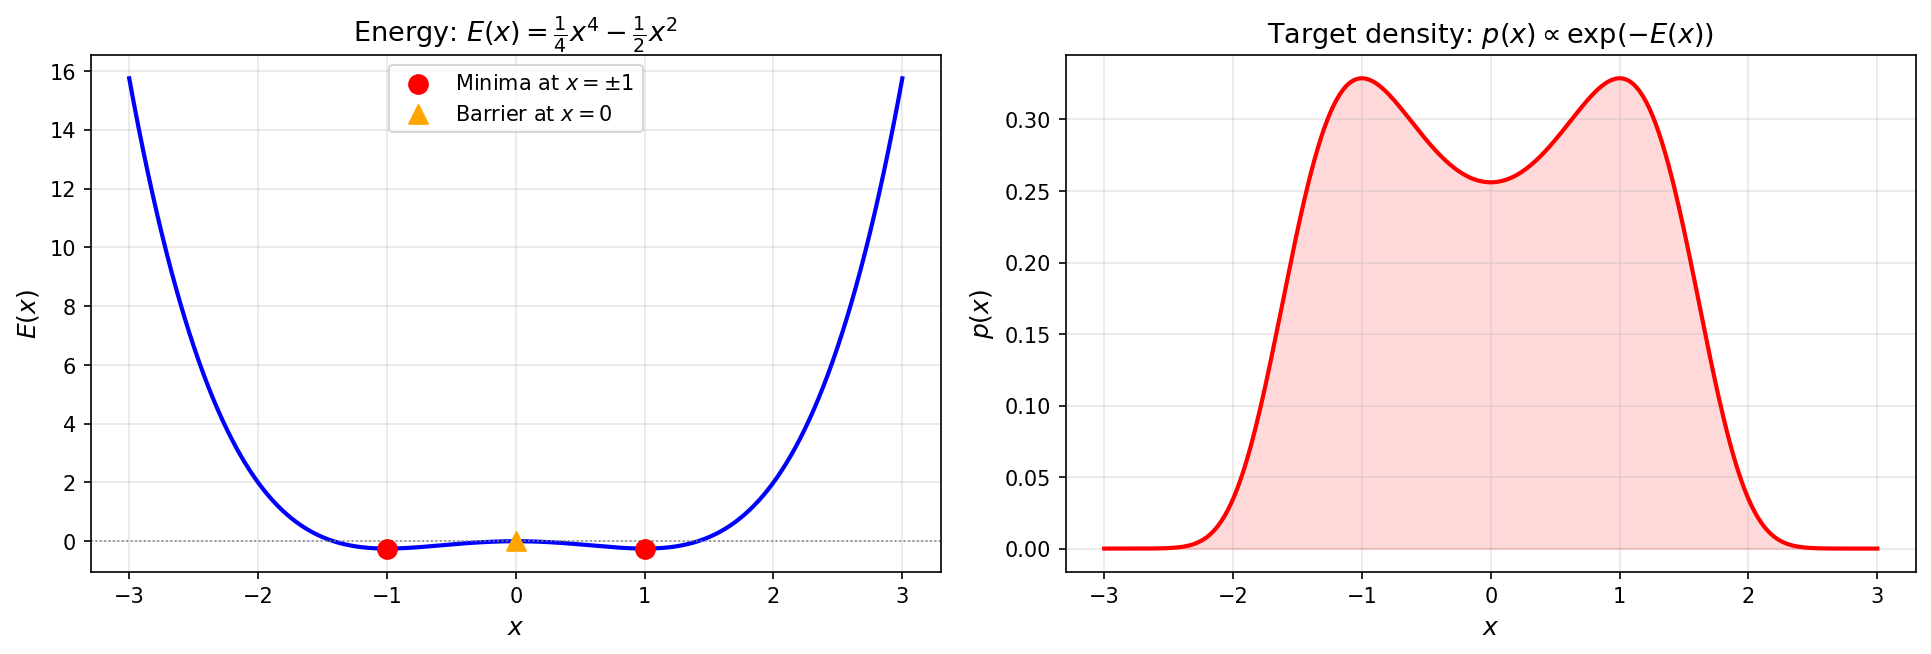
\includegraphics[width=\textwidth]{images/langevin_energy_and_density.png}
    \caption{\textbf{Left:} Energy function
             $E(x) = \tfrac{1}{4}x^4 - \tfrac{1}{2}x^2$
             with minima (red dots) and barrier (orange
             triangle).  \textbf{Right:} Corresponding
             target density $p(x) \propto \exp(-E(x))$
             --- bimodal with modes at $x = \pm 1$.}
    \label{fig:langevin_energy}
\end{figure}

\subsubsection{Sample Histogram vs True Density}

Figure~\ref{fig:langevin_hist} overlays the histogram of
Langevin samples (after burn-in) with the true density.
The close match confirms that the chain has converged and
explores both modes.

\begin{figure}[H]
    \centering
    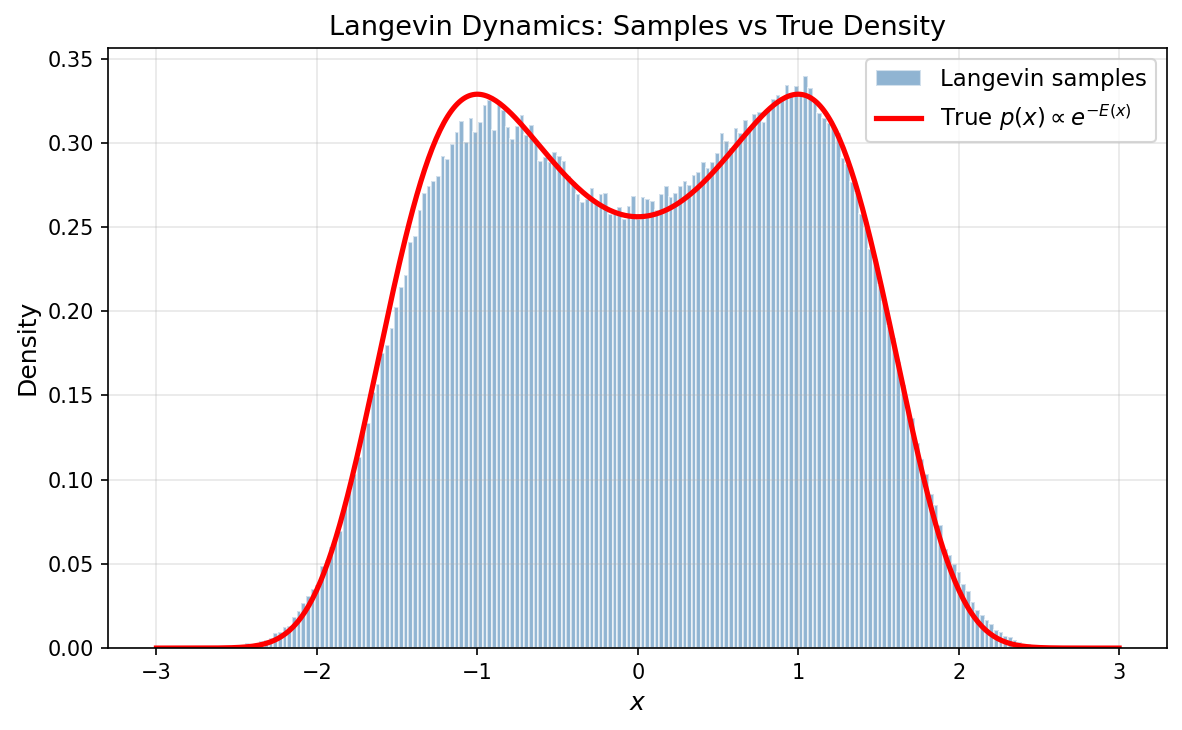
\includegraphics[width=0.75\textwidth]{images/langevin_samples_vs_density.png}
    \caption{Histogram of 499{,}000 Langevin samples
             (after 1{,}000 burn-in) overlaid with the
             true density $p(x) \propto \exp(-E(x))$.}
    \label{fig:langevin_hist}
\end{figure}

\subsubsection{Trace Plot \& Gradient Descent Comparison}

Figure~\ref{fig:langevin_trace} provides two key
visualizations:
\begin{itemize}
    \item \textbf{Left --- Trace plot}: The chain starts at
          $x_0 = 3$ and quickly drifts toward the modes at
          $\pm 1$ (gradient-driven).  It then \emph{hops}
          between the two modes---the noise enables
          transitions across the energy barrier that gradient
          descent could never make.
    \item \textbf{Right --- GD vs Langevin}: Starting from
          the same initial point $x_0 = 2.5$, gradient descent
          (orange) converges deterministically to $x = +1$ and
          stays forever.  Langevin dynamics (blue) reaches the
          same region but continues to fluctuate, eventually
          exploring both modes.
\end{itemize}

\begin{figure}[H]
    \centering
    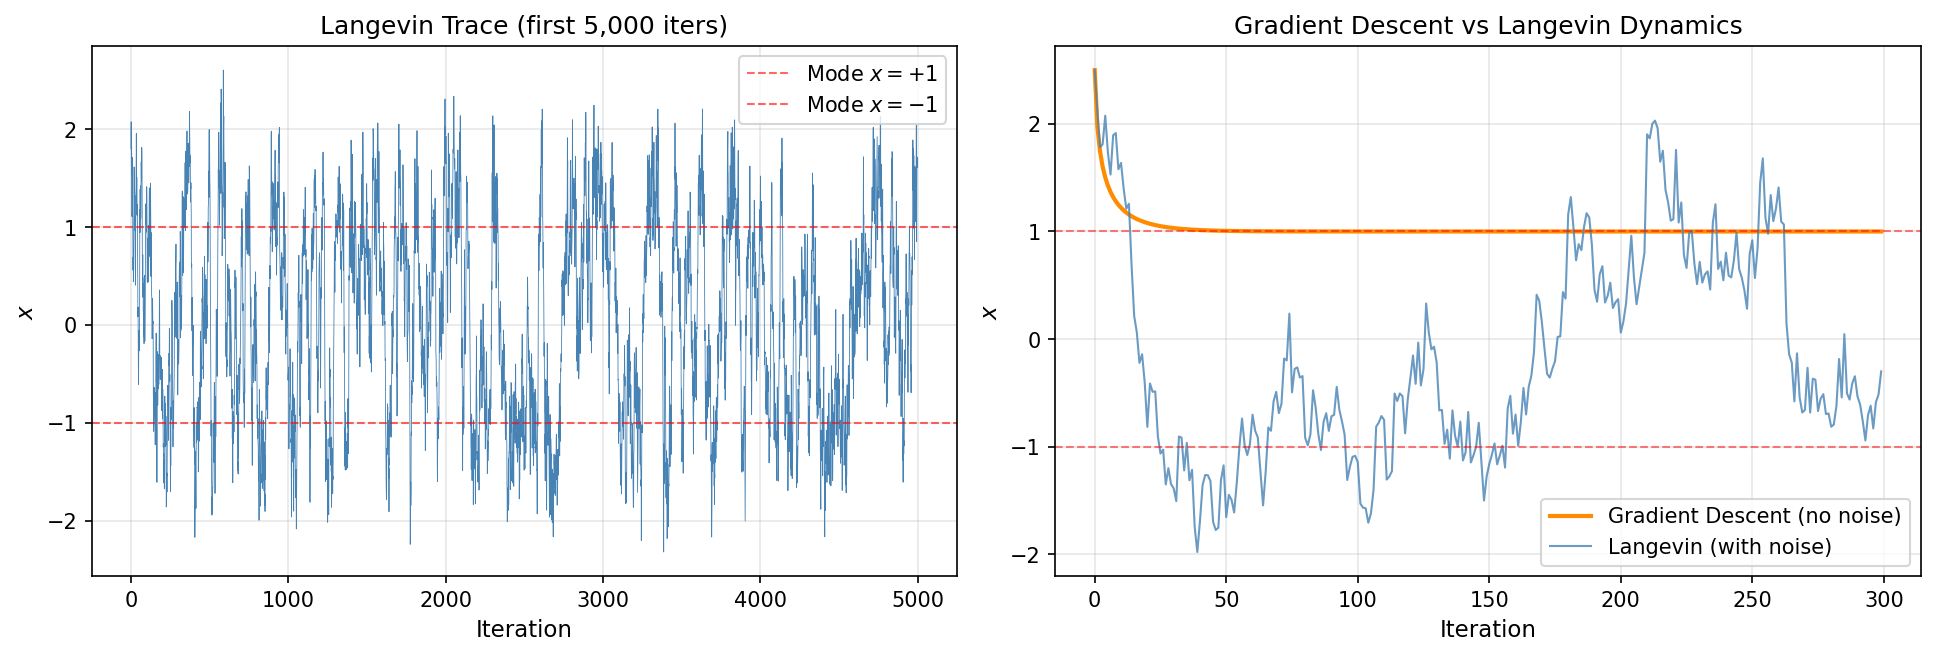
\includegraphics[width=\textwidth]{images/langevin_trace_and_gd_comparison.png}
    \caption{\textbf{Left:} Langevin trace over 5{,}000
             iterations showing mode-hopping between
             $x \approx \pm 1$.  \textbf{Right:}
             Gradient descent (deterministic, orange)
             converges to one mode; Langevin dynamics
             (stochastic, blue) explores around it.}
    \label{fig:langevin_trace}
\end{figure}

\subsubsection{Results}

\begin{table}[H]
    \centering
    \begin{tabular}{lr}
        \toprule
        \textbf{Statistic}
            & \textbf{Sample} \\
        \midrule
        Mean $x$
            & 0.026 \\
        Std $x$
            & 1.024 \\
        $\hat{E}[x^2]$
            & 1.049 \\
        \bottomrule
    \end{tabular}
    \caption{Langevin dynamics: sample statistics for the
             double-well target.  The symmetric bimodal
             density has true mean~0.}
    \label{tab:langevin_results}
\end{table}

The sample mean is close to zero (the density is symmetric)
and both modes are well-represented in the histogram.

\subsubsection{Drawbacks and Limitations}

\begin{enumerate}
    \item \textbf{Discretization bias (ULA)}.
          The update~\eqref{eq:langevin_update} is a
          \emph{discretization} of the continuous-time
          Langevin SDE.  For any finite step size $\eta > 0$,
          the stationary distribution of the discrete chain
          is \emph{not} exactly $p(x)$ but an $O(\eta)$
          approximation.  The bias vanishes only as
          $\eta \to 0$, which slows the chain.  Adding a
          Metropolis acceptance step yields the
          \textbf{Metropolis-Adjusted Langevin Algorithm
          (MALA)}, which is \emph{exact} but at the cost of
          occasional rejections.

    \item \textbf{Step-size sensitivity}.
          If $\eta$ is too large, the discretization error
          dominates and the chain may diverge.  If $\eta$ is
          too small, the gradient steps are tiny and the chain
          mixes slowly.  Finding a good $\eta$ requires
          experimentation.

    \item \textbf{Mode-hopping can be slow}.
          Transitions between well-separated modes require the
          noise to overcome the energy barrier in a single step.
          The probability of such a jump decreases
          \emph{exponentially} with the barrier height.
          For strongly multi-modal targets, tempering,
          replica exchange, or annealed methods are needed.

    \item \textbf{Requires differentiable energy}.
          The gradient $\nabla E(x)$ must exist.  This
          excludes:
          \begin{itemize}
              \item \textbf{Discrete state spaces}: probability
                    mass functions have no gradient.
              \item \textbf{Non-differentiable densities}:
                    e.g., Laplace distributions at the origin.
          \end{itemize}
          For these, gradient-free methods (MH, Gibbs) are
          needed.

    \item \textbf{Sensitive to high dimensions}.
          In very high dimensions the ``typical set'' of
          $p(x)$ is a thin shell far from the mode.
          Langevin dynamics can still work but may require
          preconditioning (scaling the gradient by the
          inverse Hessian or a mass matrix) to handle
          anisotropic targets efficiently.
\end{enumerate}

\subsubsection{Discussion}

\begin{itemize}
    \item \textbf{Gradient information}: Langevin dynamics is
          the first method in our survey that exploits
          $\nabla \log p(x)$.  This makes the proposal
          \emph{informed} rather than blind, leading to
          faster convergence than a random-walk MH chain of
          the same step size.
    \item \textbf{Connection to score-based models}:
          Modern diffusion / score-matching generative models
          (e.g., DDPM, score-based SDEs) use Langevin-type
          updates with a \emph{learned} score function
          $s_\theta(x) \approx \nabla_x \log p(x)$ to
          generate images, audio, and other data.
    \item \textbf{Comparison with other methods}:
          \begin{itemize}
              \item \emph{MH}: generic but blind proposals.
              \item \emph{Gibbs}: one-variable-at-a-time,
                    needs closed-form conditionals.
              \item \emph{Langevin}: uses gradients, works in
                    the full joint space, no need for
                    conditional decomposition.
              \item \emph{Hamiltonian Monte Carlo (HMC)}:
                    extends Langevin with momentum for
                    even more efficient exploration
                    (not covered here).
          \end{itemize}
\end{itemize}

% ══════════════════════════════════════════════════════════
\section{Summary}
\label{sec:summary}

Across all four experiments the pattern is the same: the sample average
$\hat{\mu}_N$ starts noisy for small $N$ and progressively tightens
around the true expectation as $N$ grows.

\begin{itemize}
    \item \textbf{Example 1 (Normal, $f(x)=x^2$):} Error $\approx 0.036$
          at $N=10{,}000$.
    \item \textbf{Example 2 (Exponential, $f(x)=\sin x$):} Error
          $\approx 0.005$ at $N=10{,}000$.
    \item \textbf{Example 3 (Multiple trials):} Empirical spread matches
          the $O(1/\sqrt{N})$ theoretical standard error.
    \item \textbf{Example 4 (Discrete PMF, $f(x)=x^2$):} Error
          $\approx 0.032$ at $N=10{,}000$.
    \item \textbf{Rejection Sampling (Multimodal target):} Acceptance
          rate $\approx 27.7\%$; histogram matches the true density.
    \item \textbf{Importance Sampling:} Both single-Gaussian and
          mixture proposals estimate $E_p[z^2] \approx 0.83$; the
          mixture achieves ESS~$\approx 84{,}290$ vs.\
          $\approx 49{,}542$ for the single Gaussian.
    \item \textbf{Metropolis--Hastings:} A 20{,}000-step chain with
          acceptance rate $\approx 72.6\%$ recovers both modes of a
          bimodal target; $\hat{E}[z^2] \approx 2.44$.
    \item \textbf{Gibbs Sampling:} One-variable-at-a-time updates
          from conditional distributions recover the bivariate
          Gaussian ($\rho=0.9$) with sample correlation $0.905$
          and correct marginals.
    \item \textbf{Metropolis-within-Gibbs:} Combines exact Gibbs
          steps for tractable conditionals with MH steps for
          intractable ones; successfully samples from a
          banana-shaped target with MH acceptance rate
          $\approx 64\%$.
    \item \textbf{Ancestral Sampling:} Exploits the Bayesian
          network factorization to draw exact, i.i.d.\ samples
          by traversing the DAG in topological order; recovers
          the linear Gaussian chain statistics with no burn-in
          or tuning.
    \item \textbf{Langevin Dynamics:} Gradient-guided MCMC that
          adds calibrated noise to gradient descent; recovers
          both modes of a double-well potential with
          $\hat{E}[x^2] \approx 1.05$ and sample
          mean~$\approx 0$.
\end{itemize}

These results validate that \textbf{Monte Carlo sampling} is a reliable
method for estimating expectations, that the \textbf{Law of Large
Numbers} guarantees convergence as the sample size increases,
that \textbf{rejection sampling} can accurately draw from complex
unnormalized distributions, that \textbf{importance sampling}
provides an efficient alternative when proposal design is carefully
matched to the target, that \textbf{Metropolis--Hastings} enables
sampling via local proposals without requiring a global envelope or
weight computation, that \textbf{Gibbs sampling} exploits
conditional distributions to update one variable at a time with
100\% acceptance, that \textbf{Metropolis-within-Gibbs}
bridges the gap between Gibbs and MH by handling models with
a mixture of tractable and intractable conditionals,
that \textbf{ancestral sampling} leverages the Bayesian network
structure and conditional dependencies to produce exact,
independent samples with no Markov chain overhead, and that
\textbf{Langevin dynamics} transforms gradient descent into a
sampler by adding noise scaled to the step size, exploiting the
score function $\nabla \log p(x)$ to guide proposals toward
high-density regions.

% ══════════════════════════════════════════════════════════
\section*{Reproducing the Experiments}

Monte Carlo convergence code is in
\texttt{MonteCarloSimulation.ipynb}; rejection sampling code is in
\texttt{RejectionSampling.ipynb}; importance sampling and other
sampling methods are in \texttt{Sampling.ipynb}.  Run the notebooks
end-to-end with a Python~3 kernel and \texttt{numpy}, \texttt{scipy},
\texttt{matplotlib} installed.
The images are saved to the \texttt{images/} folder automatically.

\end{document}
